\documentclass[11pt,letterpaper]{article}
\pdfoutput=1

\usepackage{jheppub}

\usepackage{amsfonts}
\usepackage{amsthm}
\usepackage{bm}
\usepackage{bbm}
\usepackage{mathtools}
\usepackage{braket}
\usepackage{booktabs}
\usepackage{tabularx}
\usepackage{threeparttable}
\usepackage{multirow}
\usepackage{float}
\usepackage{enumitem}
\usepackage{microtype}
\usepackage[T1]{fontenc}
\usepackage[utf8]{inputenc}
\usepackage{xcolor}
\usepackage{tikz}
\usepackage{pgfplots}
\usepackage{etoolbox}
\usetikzlibrary{shapes,arrows,positioning,fit,backgrounds,calc}
\pgfplotsset{compat=1.18}

\hypersetup{
    pdftitle={The Page Curve Through the Transition: An Order-One Correction to the Diagonal Approximation},
    pdfauthor={Bernd Johannes Wuebben},
    pdfsubject={Black hole information; Page curve; diagonal approximation},
    pdfkeywords={Page curve, black hole information, replica wormholes, diagonal approximation, entropy of mixing, free probability, Marchenko-Pastur law, JT gravity}
}

\newenvironment{figurenotes}{\par\footnotesize\textit{Notes:} }{\par}

\theoremstyle{plain}
\newtheorem{theorem}{Theorem}[section]
\newtheorem{proposition}[theorem]{Proposition}
\newtheorem{lemma}[theorem]{Lemma}
\newtheorem{corollary}[theorem]{Corollary}

\theoremstyle{definition}
\newtheorem{definition}[theorem]{Definition}
\newtheorem{assumption}[theorem]{Assumption}
\newtheorem{example}[theorem]{Example}

\theoremstyle{remark}
\newtheorem{remark}[theorem]{Remark}


\newcommand{\Acal}{\mathcal{A}}
\newcommand{\Bcal}{\mathcal{B}}
\newcommand{\Ccal}{\mathcal{C}}
\newcommand{\Dcal}{\mathcal{D}}
\newcommand{\Ecal}{\mathcal{E}}
\newcommand{\Fcal}{\mathcal{F}}
\newcommand{\Gcal}{\mathcal{G}}
\newcommand{\Hcal}{\mathcal{H}}
\newcommand{\Ical}{\mathcal{I}}
\newcommand{\Jcal}{\mathcal{J}}
\newcommand{\Kcal}{\mathcal{K}}
\newcommand{\Lcal}{\mathcal{L}}
\newcommand{\Mcal}{\mathcal{M}}
\newcommand{\Ncal}{\mathcal{N}}
\newcommand{\Ocal}{\mathcal{O}}
\newcommand{\Pcal}{\mathcal{P}}
\newcommand{\Qcal}{\mathcal{Q}}
\newcommand{\Rcal}{\mathcal{R}}
\newcommand{\Scal}{\mathcal{S}}
\newcommand{\Tcal}{\mathcal{T}}
\newcommand{\Ucal}{\mathcal{U}}
\newcommand{\Vcal}{\mathcal{V}}
\newcommand{\Wcal}{\mathcal{W}}
\newcommand{\Xcal}{\mathcal{X}}
\newcommand{\Ycal}{\mathcal{Y}}
\newcommand{\Zcal}{\mathcal{Z}}

\newcommand{\bzero}{\bm{0}}
\newcommand{\E}{\mathbb{E}}
\newcommand{\Var}{\text{Var}}
\newcommand{\Cov}{\text{Cov}}
\newcommand{\Corr}{\text{Corr}}
\newcommand{\R}{\mathbb{R}}
\newcommand{\N}{\mathbb{N}}
\newcommand{\Z}{\mathbb{Z}}
\newcommand{\C}{\mathbb{C}}
\newcommand{\Prob}{\mathbb{P}}

\newcommand{\F}{\mathcal{F}}
\newcommand{\G}{\mathcal{G}}

\newcommand{\bff}{\bm{f}}
\newcommand{\bh}{\bm{h}}
\newcommand{\bbeta}{\bm{\beta}}
\newcommand{\bSigma}{\bm{\Sigma}}
\newcommand{\bmu}{\bm{\mu}}

\DeclareMathOperator*{\argmin}{arg\,min}
\DeclareMathOperator*{\argmax}{arg\,max}
\DeclareMathOperator{\tr}{tr}
\DeclareMathOperator{\diag}{diag}
\DeclareMathOperator{\Tr}{Tr}

\newcommand{\convd}{\xrightarrow{d}}
\newcommand{\convp}{\xrightarrow{p}}
\newcommand{\convas}{\xrightarrow{a.s.}}

\newcommand{\ind}{\mathbbm{1}}
\newcommand{\tavg}[1]{\langle #1 \rangle_t}


\preprint{\normalfont\small February 11, 2026 \textperiodcentered{} this version: October 9, 2026}

\title{The Page Curve Through the Transition:\\
An Order-One Correction to the Diagonal Approximation}

\author{Bernd Johannes Wuebben}
\affiliation{New York, NY, USA}
\emailAdd{wuebben@gmail.com}

\abstract{In the west-coast model of black hole evaporation, the diagonal approximation computes the entropy of the radiation near the Page time by averaging the entropy of fixed-area states over the black hole's fluctuating area. We show that this approximation, written level by level, misses an order-one constant: as the area distribution becomes broad, whatever its shape, the exact entropy exceeds it by $-q\log q$, where $q$ is the canonical probability that the black hole is larger than the radiation. The constant arises because the radiation, which has no energy of its own, can resolve area sectors only through the island, and so not those in which the black hole is larger than itself. For a symmetric distribution the excess is half of $\log 2$ at the Page point and largest after it, so the exact transition is asymmetric. The proof reduces the entropy of the exact planar spectrum, a free multiplicative convolution, to a single integral. We compute the first correction and evaluate the constant in Jackiw--Teitelboim gravity. At fixed area, the two-saddle truncation misses the R\'enyi moments by Catalan factors.}


\keywords{Page curve, black hole information, replica wormholes, diagonal approximation, entropy of mixing, free probability, Marchenko--Pastur law, JT gravity}

\begin{document}

\notoc
\maketitle

\clearpage
\pagenumbering{roman}
\setcounter{page}{1}
\hrule
\tableofcontents
\afterTocSpace
\hrule
\afterTocRuleSpace
\clearpage
\pagenumbering{arabic}
\setcounter{page}{1}

\emergencystretch=2em



\section{Introduction}
\label{sec01:introduction}

Hawking's calculation~\citep{hawking1975} gives black hole radiation a thermal spectrum, and with it an entanglement entropy that grows until the black hole is gone. Unitarity requires instead that the entropy of the radiation follow the curve described by \citet{page1993entropy, page1993info}: it rises with the number of emitted quanta, turns over at the Page time, when the radiation and the black hole have equal Hilbert space dimension, and returns to zero. \citet{penington2020} and \citet{almheirietal2019} derived this curve from the gravitational path integral, using the quantum extremal surface prescription~\citep{ryutakayanagi2006, lewkowyczmaldacena2013, engelhardtwall2015}: two extremal surfaces exchange dominance at the Page time, and away from it the entropy is
\begin{equation}
\label{eq01:min_formula}
S_{\mathrm{vN}} \approx \min(S_{\mathrm{rad}}, S_{\mathrm{BH}}) .
\end{equation}
This paper is about the transition itself, where neither surface dominates.

\subsection{The transition and the diagonal approximation}
\label{subsec01:page_curve}

\citet{penington2020} observed that the exchange cannot be sharp: fluctuations of the horizon area, and of the energy of the radiation, leave no single extremal surface within a window of order $\beta\sqrt{S_{\mathrm{BH}}}$ of the Page time. The shape of the crossover was computed by \citet{marolfwangwang2020}. They decompose the state into states of fixed area and replace its entropy by the expectation of the fixed-area entropy in the ensemble the state defines, a prescription they call the \emph{diagonal approximation} and offer as a conjecture. It imports into holography a result of \citet{murthysrednicki2019} for systems obeying the eigenstate thermalization hypothesis: for an equal bipartition far from a critical point,
\begin{equation}
\label{eq01:murthy_srednicki}
S_{\mathrm{ent}} = \tfrac12\, S - \sqrt{\frac{C}{2\pi}} + O(A),
\end{equation}
with $S$ the thermodynamic entropy of the whole system, $C$ its heat capacity and $A$ the area of the boundary between the halves. Applied to a black hole whose entropy has variance $\sigma^2 = C_V$, the diagonal approximation lowers the entropy at the Page time by $\sigma/\sqrt{2\pi}$ and spreads the transition over a range of order $\sigma$, in agreement with the canonical-ensemble calculation of \citet{pssyetal2022}.

The diagonal approximation is accurate at the order at which it was formulated, $O(G_N^{-1/2})$. Below that order it has not been evaluated. \citet{marolfwangwang2020} drop the entropy of mixing between area sectors as $O(\log G_N)$ and leave the remainder at $O(G_N^0)$; \citet{akerspenington2021}, \citet{chengetal2024} and \citet{peningtonrath2025} derive or bound the prescription to within $O(\log G_N)$ or $O(\log n)$, the last for R\'enyi entropies. In one model the exact answer is available. In the model of Penington, Shenker, Stanford and Yang~\citep{pssyetal2022}, the \emph{west-coast model}, the planar radiation spectrum in the canonical ensemble is determined by a resolvent equation that they derive and solve numerically, and they observe that an approximation to it agrees with the average of the microcanonical answer to within $O(1)$. \citet{wang2023} and \citet{chengetal2024} identify the spectrum as a free multiplicative convolution. This paper evaluates the order-one difference between the exact planar entropy and the diagonal approximation.

\subsection{The result}
\label{subsec01:novel_results}

Write $S_{\mathrm{planar}}$ for the exact planar entropy of the radiation and $S_{\mathrm{diag}}$ for the diagonal approximation, in the form in which each sector of the black hole carries its share of the black hole's von Neumann entropy (Section~\ref{subsec04:diagonal}); this form is free of any choice of area windows and is correct well before and well after the Page time. The windowed form of \citet{marolfwangwang2020} does not determine the terms of order one, because the entropy of mixing that it drops depends on the windows at order $\log G_N$. Both are determined by the distribution of the black hole's eigenvalue levels relative to the radiation. Let $q$ be the canonical weight of the levels larger than the radiation, those at which a fixed-area black hole would have dimension greater than that of the radiation; $q$ falls from one to zero as the radiation grows.

\begin{quote}
\textbf{Theorem} (Section~\ref{sec45:exact_correction}). As the area distribution becomes broad on the scale of one nat,
\begin{equation}
\label{eq01:main}
S_{\mathrm{planar}} - S_{\mathrm{diag}} \;\longrightarrow\; -\,q\log q .
\end{equation}
For a symmetric area distribution $q \to \tfrac12$ at the Page point and the correction is $\tfrac12\log 2$; over all $q$ it is largest, equal to $1/e$, at $q = 1/e$, after the Page time.
\end{quote}

The mechanism is simple. Levels in which the black hole is smaller than the radiation occupy nearly orthogonal subspaces of the radiation, and the diagonal approximation counts their entropy of mixing correctly. Levels in which the black hole is larger than the radiation each fill the whole radiation space; the radiation cannot tell them apart, and together they lay a flat floor of height $q$ under its spectrum, whose entropy $-q\log q$ the diagonal approximation misses. \citet{marolfwangwang2020} anticipate the distinction: the radiation states of different area sectors are guaranteed to be orthogonal only when the black hole is smaller than the radiation, and they treat all sectors as orthogonal as an additional assumption. The constant is the cost of that assumption. It arises because the radiation of the west-coast model has no energy of its own and resolves area sectors only through the island, which reconstructs the sector only when the black hole is the smaller of the two; where the radiation records the sector directly, as for an energy eigenstate of a closed system, all sectors are orthogonal and no floor forms~\citep{murthysrednicki2019}. The constant is implicit in the canonical-ensemble analysis of \citet{pssyetal2022}, whose approximate entropy contains the block term, and in the two-component mixtures of \citet{akerspenington2021}; the present paper evaluates it, proves that it is the limit of the error of the diagonal approximation for every sufficiently broad area distribution, and computes the approach to the limit.

The specific results are these.
\begin{itemize}
\item \textbf{A one-dimensional representation} of the exact planar entropy (Proposition~\ref{thm45:representation}). On the negative real axis the self-consistent equation for the Cauchy transform can be solved explicitly for the spectral parameter, which reduces the entropy, and its difference from the diagonal approximation, to a single quadrature with no fixed-point iteration and no Stieltjes inversion.
\item \textbf{The broad-distribution limit}~\eqref{eq01:main} (Theorem~\ref{thm45:limit}), for any family of area distributions that spreads, with a counterexample showing that the spreading condition is needed.
\item \textbf{The first correction} for area distributions with a smooth density: the gap falls short of $-q\log q$ by $f(0)\,(\pi^2/6 + \log q + \tfrac12\log^2 q)$, where $f$ is the density of the distance of a level from the radiation (Section~\ref{subsec45:first_order}; derived formally, and confirmed numerically for Gaussian laws to $\sigma = 400$ and for the JT law). For a Gaussian distribution of width $\sigma$ at the Page point, $S_{\mathrm{planar}} - S_{\mathrm{diag}} = \tfrac12\log 2 - K/\sigma + O(\sigma^{-2})$ with $K = (\pi^2/6 - \log 2 + \tfrac12\log^2 2)/\sqrt{2\pi}$. The exact deficit at the Page point is then $-\sigma/\sqrt{2\pi} + \tfrac12\log 2 + O(1/\sigma)$: the diagonal approximation has the leading term, misses the constant, and gets the $1/\sigma$ coefficient wrong by a factor of about $2.2$.
\item \textbf{The JT model} (Section~\ref{sec05:exact_jt}). In the west-coast model with the JT area distribution, the correction is $0.20$ nats at $\beta = 2\pi$ and approaches its limit at high temperature as $0.48/\sigma$, as the first correction predicts. The area distribution is the JT one only when the brane tension is large, $\mu \gg 2\pi/\beta$, and its pure-JT form needs in addition $\sigma/(\beta\mu) \ll 1$.
\end{itemize}

The fixed-area input, assembled from known ingredients, also yields the following. Summing all non-crossing permutations, rather than the two dominant saddles, gives the Marchenko--Pastur law, and at the Page time the two-saddle truncation underestimates the $n$th R\'enyi moment by the factor $C_n/2$, where $C_n$ is the $n$th Catalan number (Section~\ref{subsec02:two_saddle}); the ratio follows at once from the Catalan count of \citet{pssyetal2022} and \citet{marolfwangwang2020}, and we record it because it measures what the truncation discards. In consequence the R\'enyi entropies at genus zero broaden through the transition as $n$ grows, where the two-saddle answer would make them sharpen (Section~\ref{subsec05:renyi}). The fixed-area deficit $-\tfrac12 e^{-|\Delta|}$ is exact on the planar spectrum, as \citet{pssyetal2022} observe; the value is classical, and we give a short proof in the normalization used here (Proposition~\ref{prop03:exact_deficit}). The genus-one permutations relative to a long cycle number $\binom{2n-2}{n-1}(n-1)(n-2)/12$, a classical count~\citep{goupilschaeffer1998}, which bounds what the planar analysis omits at $O(e^{-2S_0})$.

\subsection{Relation to prior work}
\label{subsec01:prior_work}

\paragraph{The broadened curve.} The correction set by the square root of the heat capacity was first seen in quantum many-body systems. \citet{vidmarrigol2017} proved, for random states at fixed particle number divided into equal halves away from half filling, that an upper bound on the average entanglement entropy falls below its maximal value by an amount growing as the square root of the subsystem volume, and found numerically that eigenstates of chaotic Hamiltonians follow it; at half filling the deviation vanishes. \citet{murthysrednicki2019} derived~\eqref{eq01:murthy_srednicki} for generic systems obeying the eigenstate thermalization hypothesis, together with the crossover function, the width $\sim\sqrt{C}$ and the generalization to further conserved charges, under the explicit assumption that the system is far from a critical point. They also note that the Marchenko--Pastur law contributes the Page correction $-e^{S_{\min}}/2e^{S_{\max}}$, which is the fixed-area deficit $-\tfrac12 e^{-|\Delta|}$ of the present paper, and neglect it as being of order one. \citet{marolfwangwang2020} brought the result into holography as the diagonal approximation; their Eq.~(3.14), for a quadratic area distribution, is the broadened curve recovered in Section~\ref{subsec04:gaussian_broadening}. \citet{pssyetal2022} obtained the corresponding $O(G_N^{-1/2})$ correction in the west-coast model itself, and \citet{penington2020} estimated the width.

\paragraph{The exact planar spectrum.} \citet{pssyetal2022} derive the resolvent equation for the radiation spectrum of their model in the canonical ensemble, exact at planar order (their Eq.~(2.34)), solve it numerically (their Fig.~7), and analyse the transition at small $\beta$ in their Appendix~F. \citet{wang2023} observes that the replica sum is combinatorially a free multiplicative convolution, $\nu_{\tilde r} = \nu_r \boxtimes \mu_{\nu_b}$, with the gravitational partition functions entering as the free cumulants of a free compound Poisson law; he argues that the replica trick is then a well-posed Hausdorff moment problem and gives an algorithm for the convolution. \citet{chengetal2024} reach the same structure from random tensor networks: their Theorem~3.4 gives $\mathrm{MP}(1)\boxtimes\mu_{\gamma_1}\boxtimes\mu_{\gamma_2}$ for two competing minimal cuts, and their Appendix~A.3 sketches the JT computation with branes. At fixed area and with flat matter the law collapses to Marchenko--Pastur, the case of Section~\ref{sec03:free_probability}. We use this description of the planar spectrum and do not rederive it.

\paragraph{The error of the diagonal approximation.} \citet{marolfwangwang2020} support the diagonal approximation by consistency with \citet{murthysrednicki2019} and \citet{pssyetal2022}, flag the orthogonality of sectors as an additional assumption, note that it need not hold for sectors in which the black hole is larger than the radiation, and expect the prescription to fail for carefully chosen non-generic states. \citet{akerspenington2021} derive it to within $O(\log G_N)$, and in their Section~4.3, with details in their Appendix~A, treat a two-component mixture whose entropy contains, in the appropriate regime, the block term $-q\log q$. \citet{pssyetal2022} write the canonical radiation density matrix as its projection onto the largest eigenvalues plus a multiple of the identity that collects the rest of the black hole spectrum; their shifted thermal spectrum (their Eq.~(F.56)), which they estimate to be accurate to $O(\beta)$, contains the corresponding block, and they note that their approximation agrees with the average of the microcanonical answer to within $O(1)$, without evaluating the difference. \citet{akersetal2022} call the weight of that remainder the pre-Page probability. \citet{chengetal2024} show for random tensor networks that the entropy is given by the diagonal formula up to $O(\log n)$, and \citet{peningtonrath2025} derive the diagonal approximation for R\'enyi entropies up to $O(\log G_N)$. To our knowledge the order-one error has not been evaluated: it is implicit in the shifted thermal spectrum of \citet{pssyetal2022} but left inside the $O(1)$ remainder of their Page-point result. Its value, its independence of the shape of the area distribution, and the proof that it is the limit for broad distributions are new here.


\subsection{Outline}
\label{subsec01:outline}

Section~\ref{sec02:pssy_model} reviews the west-coast model and its genus-zero replica sum, and quantifies the failure of the two-saddle truncation. Section~\ref{sec03:free_probability} identifies the fixed-area spectrum as Marchenko--Pastur, states the exact fixed-area deficit, and states the exact planar spectrum in the canonical ensemble. Section~\ref{sec04:area_fluctuations} states the diagonal approximation, fixes the form in which it is compared, and records its closed form for Gaussian area distributions. Section~\ref{sec45:exact_correction} contains the main results: the representation, the limit, its mechanism and its first correction. Section~\ref{sec05:exact_jt} applies them to the JT model and records the R\'enyi entropies at fixed area. Section~\ref{sec06:discussion} discusses what the correction means and what remains open. The appendices give the permutation combinatorics, the free-probability derivations, the Gaussian integrals, the proofs of Section~\ref{sec45:exact_correction}, and the numerical methods.

\section{The West-Coast Model and Its Genus-Zero Replica Sum}
\label{sec02:pssy_model}

This section reviews the model of \citet{pssyetal2022} and evaluates its replica sum at genus zero. Retaining only the two distinguished saddles, the fully disconnected and the fully connected replica geometries, discards the partially connected ones. At the Page time this underestimates the $n$th R\'enyi moment by the factor $C_n/2$, where $C_n$ is the $n$th Catalan number, so the two-saddle answer cannot be continued to $n \to 1$ at the transition. The full genus-zero sum runs over the non-crossing permutations and is organized by the Narayana numbers.

\subsection{Setup: JT gravity with end-of-the-world branes}
\label{subsec02:setup}

The model of Penington, Shenker, Stanford and Yang~\citep{pssyetal2022}, known as the \emph{west-coast model}, couples Jackiw--Teitelboim (JT) gravity~\citep{jackiwteitelboim1985,saadetal2019} to $k$ flavors of end-of-the-world (EOW) branes. The black hole interior is a disk whose boundary carries a brane of flavor $i \in \{1, \ldots, k\}$. In the fixed-area version of the model the black hole Hilbert space has dimension $L = e^{S_0}$.

The state of the black hole and the radiation is
\begin{equation}
\label{eq02:psi_state}
|\psi\rangle = \frac{1}{\sqrt{Z}} \sum_{i=1}^{k} |\psi_i\rangle_{\mathrm{BH}} \otimes |i\rangle_{\mathrm{rad}},
\end{equation}
where $|\psi_i\rangle$ is the black hole state with a brane of flavor $i$, the $|i\rangle_{\mathrm{rad}}$ form an orthonormal basis of the radiation Hilbert space of dimension $k$, and $Z = \sum_i \langle\psi_i|\psi_i\rangle$. Tracing out the black hole gives the radiation density matrix
\begin{equation}
\label{eq02:rho_rad}
\rho_{\mathrm{rad}} = \frac{1}{Z} \sum_{i,j=1}^{k} \langle\psi_j|\psi_i\rangle \, |i\rangle\langle j|.
\end{equation}
The overlaps $\langle\psi_j|\psi_i\rangle$ are computed by the gravitational path integral. On the disk, $\langle\psi_j|\psi_i\rangle \propto \delta_{ij}$, so that $\rho_{\mathrm{rad}} = \mathbb{1}_k/k$ is maximally mixed; geometries with more boundaries correlate the overlaps and carry the entanglement structure. The object of interest is the von Neumann entropy
\begin{equation}
\label{eq02:svn_def}
S_{\mathrm{vN}} = -\mathrm{Tr}(\rho_{\mathrm{rad}} \log \rho_{\mathrm{rad}}),
\end{equation}
which the replica trick computes as $S_{\mathrm{vN}} = -\lim_{n \to 1} \partial_n \mathrm{Tr}(\rho_{\mathrm{rad}}^n)$.

\subsection{The replica path integral}
\label{subsec02:replica}

For integer $n \geq 2$,
\begin{equation}
\label{eq02:trace_rho_n}
\mathrm{Tr}(\rho_{\mathrm{rad}}^n) = \frac{1}{Z^n} \sum_{i_1, \ldots, i_n} \langle\psi_{i_2}|\psi_{i_1}\rangle \langle\psi_{i_3}|\psi_{i_2}\rangle \cdots \langle\psi_{i_1}|\psi_{i_n}\rangle .
\end{equation}
The gravitational path integral sums over all ways of connecting the $n$ replicas by wormholes~\citep{almheirietal2020,pssyetal2022}, and in the fixed-area model the result is~\citep{pssyetal2022}
\begin{equation}
\label{eq02:pssy_master}
\mathrm{Tr}(\rho_{\mathrm{rad}}^n) = (kL)^{-n} \sum_{\sigma \in S_n} k^{\#(\tau^{-1}\sigma)} \, L^{\#(\sigma)},
\end{equation}
where $\tau = (1\,2\,\cdots\,n)$ is the cyclic permutation fixed by the trace and $\#(\cdot)$ is the number of cycles of a permutation. The factor $k^{\#(\tau^{-1}\sigma)}$ counts the closed loops of radiation indices, and $L^{\#(\sigma)}$ counts the black hole index loops, one for each disk of the replica geometry. Equation~\eqref{eq02:pssy_master} is the moment formula of a Haar-random pure state on $\mathcal{H}_k \otimes \mathcal{H}_L$ at leading order in $1/(kL)$~\citep{lubkin1978,lloydpagels1988,page1993entropy}.

\subsection{The genus expansion and non-crossing permutations}
\label{subsec02:genus}

A permutation $\sigma$ contributes at genus
\begin{equation}
\label{eq02:genus_formula}
g(\sigma) = \frac{n + 1 - \#(\sigma) - \#(\tau^{-1}\sigma)}{2},
\end{equation}
suppressed by $L^{-2g}$ relative to genus zero. The genus-zero condition
\begin{equation}
\label{eq02:genus_zero_condition}
\#(\sigma) + \#(\tau^{-1}\sigma) = n + 1
\end{equation}
is the geodesic condition: it holds exactly when $\sigma$ lies on a geodesic from the identity to $\tau$ in the Cayley graph of $S_n$ generated by transpositions. The permutations satisfying it are the non-crossing permutations $S_{\mathrm{NC}}(n)$, which are in bijection with the lattice $\mathrm{NC}(n)$ of non-crossing partitions of $\{1, \ldots, n\}$ by sending a permutation to the partition into its cycles~\citep{biane1997, nicaspeicher2006}. There are $C_n = \frac{1}{n+1}\binom{2n}{n}$ of them.

Write $\gamma = k/L$ for the ratio of the radiation and black hole dimensions. On $S_{\mathrm{NC}}(n)$ the condition~\eqref{eq02:genus_zero_condition} gives
\begin{equation}
\label{eq02:contribution_nc}
(kL)^{-n}\, k^{\#(\tau^{-1}\sigma)} L^{\#(\sigma)} = \gamma^{\,1 - \#(\sigma)}\, L^{1-n} = k^{1-n}\, \gamma^{\,n - \#(\sigma)},
\end{equation}
and summing,
\begin{equation}
\label{eq02:trace_genus_zero}
\mathrm{Tr}(\rho_{\mathrm{rad}}^n)\big|_{g=0} = k^{1-n} \, M_n(\gamma), \qquad M_n(\gamma) = \sum_{\sigma \in S_{\mathrm{NC}}(n)} \gamma^{\,n - \#(\sigma)} .
\end{equation}
This holds for every value of $\gamma$, on either side of the Page time. Section~\ref{sec03:free_probability} identifies $M_n(\gamma)$ as the $n$th moment of the Marchenko--Pastur law of ratio $\gamma$. At $n = 2$, $\mathrm{Tr}(\rho_{\mathrm{rad}}^2) = k^{-1}(1+\gamma) = 1/k + 1/L$, the standard purity.

\subsection{Narayana decomposition}
\label{subsec02:narayana}

Exactly $N(n,j)$ of the permutations in $S_{\mathrm{NC}}(n)$ have $j$ cycles, where
\begin{equation}
\label{eq02:narayana_def}
N(n,j) = \frac{1}{n} \binom{n}{j} \binom{n}{j-1}
\end{equation}
is the Narayana number~\citep{nicaspeicher2006}, so that
\begin{equation}
\label{eq02:moment_narayana}
M_n(\gamma) = \sum_{j=1}^{n} N(n,j) \, \gamma^{\,n-j} ,
\end{equation}
the decomposition used by \citet{pssyetal2022} in their Appendix~E. Table~\ref{tab02:narayana} lists $N(n,j)$ for small $n$; each row sums to $C_n$.

\begin{table}[htbp]
\centering
\caption{Narayana numbers $N(n,j)$ for $n = 2, 3, 4, 5$. Each row sums to the Catalan number $C_n$.}
\label{tab02:narayana}
\begin{tabular}{c|ccccc|c}
\hline
$n$ & $N(n,1)$ & $N(n,2)$ & $N(n,3)$ & $N(n,4)$ & $N(n,5)$ & $\sum_j = C_n$ \\
\hline
2 & 1 & 1 & --- & --- & --- & 2 \\
3 & 1 & 3 & 1 & --- & --- & 5 \\
4 & 1 & 6 & 6 & 1 & --- & 14 \\
5 & 1 & 10 & 20 & 10 & 1 & 42 \\
\hline
\end{tabular}
\end{table}

The symmetry $N(n,j) = N(n, n+1-j)$ is Kreweras complementation, $\sigma \mapsto \sigma^{-1}\tau$, which maps $S_{\mathrm{NC}}(n)$ to itself and sends $j$ cycles to $n+1-j$~\citep{nicaspeicher2006}. In terms of the moments it reads $\gamma^{\,n-1} M_n(1/\gamma) = M_n(\gamma)$, which is the statement $k^{1-n}M_n(k/L) = L^{1-n}M_n(L/k)$: the radiation and the black hole of a pure state have the same R\'enyi moments.

At the Page time, $\gamma = 1$, the moment is the Catalan number:
\begin{equation}
\label{eq02:moment_page_time}
M_n(1) = \sum_{j=1}^{n} N(n,j) = C_n .
\end{equation}

\subsection{The two-saddle approximation and its failure}
\label{subsec02:two_saddle}

The saddle-point treatment keeps two of the $C_n$ non-crossing permutations: the identity, the fully disconnected geometry with $n$ cycles and weight $\gamma^0 = 1$, and $\tau$, the fully connected geometry with one cycle and weight $\gamma^{\,n-1}$. It gives
\begin{equation}
\label{eq02:two_saddle}
\mathrm{Tr}(\rho_{\mathrm{rad}}^n)_{\text{two-saddle}} = k^{1-n}(1 + \gamma^{\,n-1}) = k^{1-n} + L^{1-n},
\end{equation}
the familiar exchange of dominance: the identity dominates for $\gamma < 1$ and the cyclic permutation for $\gamma > 1$. At the Page time
\begin{equation}
\label{eq02:two_saddle_page}
\mathrm{Tr}(\rho_{\mathrm{rad}}^n)_{\text{two-saddle}}\big|_{\gamma=1} = 2 L^{1-n},
\qquad
\mathrm{Tr}(\rho_{\mathrm{rad}}^n)\big|_{g=0,\,\gamma=1} = C_n \, L^{1-n},
\end{equation}
so that
\begin{equation}
\label{eq02:catalan_ratio}
\boxed{\frac{\mathrm{Tr}(\rho_{\mathrm{rad}}^n)\big|_{g=0}}{\mathrm{Tr}(\rho_{\mathrm{rad}}^n)_{\text{two-saddle}}}\Bigg|_{\gamma=1} = \frac{C_n}{2}}
\end{equation}
with values
\begin{equation}
\label{eq02:ratio_values}
\frac{C_n}{2} = 1,\; 2.5,\; 7,\; 21,\; 66,\; 214.5,\; \ldots \qquad (n = 2, 3, 4, 5, 6, 7, \ldots),
\end{equation}
growing as $4^n/(2\sqrt{\pi}\, n^{3/2})$. The two-saddle approximation is exact only for the purity, $n = 2$. The $C_n - 2$ permutations it discards are the partially connected replica geometries, and at the Page time their total weight exceeds that of the two extreme geometries for every $n \geq 3$. They are what turns the cusp of the two-saddle Page curve into a smooth crossover; the planar resolvent of \citet{pssyetal2022} retains them by construction, and the ratio $C_n/2$ measures, moment by moment, what the truncation discards. The ratio follows at once from the Catalan count of the planar geometries at the Page time, which \citet{pssyetal2022} give in their Appendix~E and \citet{marolfwangwang2020} use in their Eq.~(3.9) for the R\'enyi entropies at equal areas; we record it because it quantifies the truncation.


Figure~\ref{fig02:page_transition} summarizes the section: the entropy through the transition, its deficit from the saddle-point answer $\min(\log k, \log L)$, the R\'enyi entropies with and without the partially connected geometries, and the ratio $C_n/2$.

\begin{figure}[htbp]
\centering
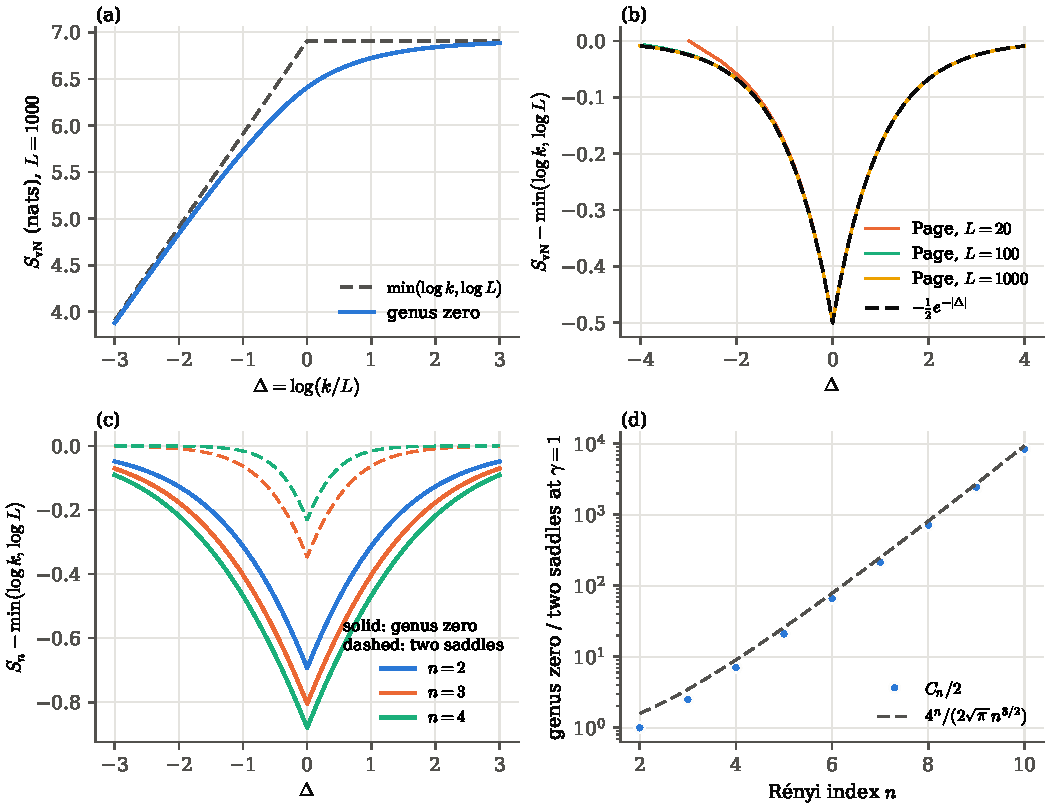
\includegraphics[width=0.95\textwidth]{figures/output/fig02_transition.pdf}
\caption{The Page transition at fixed area. (a) The genus-zero von Neumann entropy against $\Delta = \log\gamma = S_{\mathrm{rad}} - S_{\mathrm{BH}}$, with the saddle-point answer $\min(\log k, \log L)$. (b) The deficit $S_{\mathrm{vN}} - \min(\log k, \log L)$: Page's finite-dimensional formula for several $L$ and the genus-zero limit $-\tfrac12 e^{-|\Delta|}$. (c) R\'enyi entropies at genus zero (solid) and in the two-saddle approximation (dashed); they agree for $n = 2$ and separate for $n \geq 3$. (d) The ratio $C_n/2$ of the genus-zero to the two-saddle R\'enyi moment at the Page time.}
\label{fig02:page_transition}
\end{figure}

\section{Free Probability and the Planar Spectrum}
\label{sec03:free_probability}

The genus-zero moments of Section~\ref{sec02:pssy_model} are a sum over non-crossing permutations, which is the combinatorial setting of free probability~\citep{voiculescu1991, nicaspeicher2006}. This section identifies the spectrum of the radiation at fixed area as the Marchenko--Pastur law, records the exact value of its entropy, and then states the exact planar spectrum in the canonical ensemble, in which the black hole energy, and with it the area, fluctuates: it is determined by a resolvent equation of \citet{pssyetal2022} and identified by \citet{wang2023} as a free multiplicative convolution. That planar spectrum is the exact side of the comparison carried out in Section~\ref{sec45:exact_correction}.

\subsection{The moment--cumulant relation on NC(n)}
\label{subsec03:moment_cumulant}

The moments $M_n$ of a probability law and its free cumulants $\kappa_m$ are related by a sum over the non-crossing partitions~\citep{nicaspeicher2006}:
\begin{equation}
\label{eq03:moment_cumulant}
M_n = \sum_{\pi \in \mathrm{NC}(n)} \prod_{B \in \pi} \kappa_{|B|} .
\end{equation}
Under the bijection between $S_{\mathrm{NC}}(n)$ and $\mathrm{NC}(n)$ of Section~\ref{subsec02:genus}, a permutation with $\#(\sigma)$ cycles corresponds to a partition with $\#(\sigma)$ blocks, and the genus-zero weight $\gamma^{\,n-\#(\sigma)}$ of~\eqref{eq02:trace_genus_zero} factorizes over blocks as $\prod_B \gamma^{|B|-1}$. The moments $M_n(\gamma)$ therefore have free cumulants
\begin{equation}
\kappa_m = \gamma^{\,m-1} \qquad (m\ge 1),
\label{eq03:free_cumulants_scaled}
\end{equation}
with $\kappa_1 = M_1 = 1$ fixed by $\mathrm{Tr}\,\rho_{\mathrm{rad}} = 1$. A free Poisson law with rate $\lambda$ and jump size $a$ has free cumulants $\kappa_m = \lambda a^m$; here $\kappa_m = (1/\gamma)\,\gamma^m$, so $\lambda = 1/\gamma$ and $a = \gamma$, and the normalization $\kappa_1 = \lambda a = 1$ is automatic. The $R$-transform $R(z) = \sum_{m\ge1}\kappa_m z^{m-1}$ is
\begin{equation}
R(z) = \sum_{m=1}^{\infty}(\gamma z)^{m-1} = \frac{1}{1-\gamma z},
\label{eq03:R_transform_scaled}
\end{equation}
the free Poisson form $\lambda a/(1 - a z)$ in the density-matrix normalization.

\begin{remark}
\label{rem03:free_poisson}
The planar restriction reproduces the non-crossing moment--cumulant combinatorics term by term, and the brane weights select the free cumulants $\gamma^{m-1}$. This is a statement about the spectral law of a single operator; it does not by itself involve freeness, which is a relation between subalgebras characterized by the vanishing of mixed free cumulants. Freeness proper enters in the canonical ensemble of Section~\ref{subsec03:canonical}, where the radiation spectrum is a free multiplicative convolution of the gravitational and matter spectra~\citep{wang2023}.
\end{remark}

\subsection{The Marchenko--Pastur law}
\label{subsec03:marchenko_pastur}

Inverting the Cauchy transform of~\eqref{eq03:R_transform_scaled} (Appendix~\ref{app:free_probability}) gives the Marchenko--Pastur law~\citep{marchenkopastur1967} of mean one and ratio $\gamma$,
\begin{equation}
\label{eq03:marchenko_pastur}
f_{\mathrm{MP}}(x; \gamma) = \frac{\sqrt{(a_+ - x)(x - a_-)}}{2\pi\gamma x} \quad \text{for } x \in [a_-, a_+], \qquad a_\pm = (1 \pm \sqrt{\gamma})^2,
\end{equation}
together with an atom of mass $1 - 1/\gamma$ at $x = 0$ when $\gamma > 1$, which accounts for the $k - L$ zero eigenvalues of $\rho_{\mathrm{rad}}$ when $k > L$. It is the limiting spectral law of a normalized Wishart matrix: the eigenvalues of $k\rho_{\mathrm{rad}}$ are distributed as $f_{\mathrm{MP}}(\,\cdot\,;\gamma)$ in the limit of large $k$ and $L$ at fixed $\gamma$, as for a Haar-random pure state~\citep{lubkin1978, lloydpagels1988, page1993entropy}.

Since $\rho_{\mathrm{rad}}$ is $k \times k$ with eigenvalues $x_i/k$, where the $x_i$ are distributed as $f_{\mathrm{MP}}$ including the atom,
\begin{equation}
\label{eq03:svn_from_mp}
S_{\mathrm{vN}} = -\sum_i \frac{x_i}{k} \log \frac{x_i}{k} = \log k - \int x \log x \, d\nu_\gamma(x),
\end{equation}
where $\nu_\gamma$ denotes the law~\eqref{eq03:marchenko_pastur}. The atom contributes nothing to the integral. Equation~\eqref{eq03:svn_from_mp} holds for every $\gamma$; it is $\log k$, and not $\log\min(k,L)$, that appears, because the integral runs over all $k$ eigenvalues.

\subsection{Continuation in the R\'enyi index}
\label{subsec03:carlson}

The path integral defines $\mathrm{Tr}(\rho_{\mathrm{rad}}^n) = k^{1-n}M_n(\gamma)$ at integer $n \ge 2$, while
\begin{equation}
\label{eq03:replica_trick}
S_{\mathrm{vN}} = -\lim_{n \to 1} \partial_n \mathrm{Tr}(\rho_{\mathrm{rad}}^n) = \log k - \lim_{n \to 1} \partial_n M_n(\gamma)
\end{equation}
requires a continuation in $n$. The Marchenko--Pastur moments $M_n(\gamma) = \int x^n\, d\nu_\gamma(x)$ supply one: the integral agrees with the Narayana polynomials at positive integers, is analytic in a right half-plane, and satisfies $|M_{1+z}(\gamma)| \le a_+^{\mathrm{Re}\,z}$ for $\mathrm{Re}\,z \ge 0$, because $\nu_\gamma$ has mean one and is supported on $[0, a_+]$; in particular it is bounded on the line $\mathrm{Re}\,z = 0$. Carlson's theorem~\citep{carlson1914} asserts that a function of exponential type in $\mathrm{Re}\,z \ge 0$, whose type along the imaginary axis is less than $\pi$, and which vanishes at the non-negative integers, vanishes identically. The continuation is therefore unique, for every $\gamma$, among continuations of exponential type that are bounded on the line $\mathrm{Re}\,n = 1$ (Appendix~\ref{subsecB:carlson}). \citet{wang2023} argues more generally that the gravitational replica trick is a well-posed Hausdorff moment problem. The R\'enyi entropies at real $n > 0$ are
\begin{equation}
\label{eq03:renyi_real_n}
S_n(\gamma) = \log k + \frac{1}{1-n}\log M_n(\gamma) .
\end{equation}

\subsection{The fixed-area deficit}
\label{subsec03:pssy_scaling}

Let $\Delta = \log\gamma = S_{\mathrm{rad}} - S_{\mathrm{BH}}$ be the distance from the Page time in entropy units, with $S_{\mathrm{rad}} = \log k$ and $S_{\mathrm{BH}} = \log L$. The genus-zero entropy is
\begin{equation}
\label{eq03:pssy_scaling_function}
S_{\mathrm{vN}} = \log\min(k,L) + \mathcal{F}(\Delta), \qquad
\mathcal{F}(\Delta) = -\frac{1}{2} e^{-|\Delta|} .
\end{equation}
The value is classical. It is the large-dimension limit of the average entanglement entropy of a random bipartite pure state, studied by \citet{lubkin1978} and \citet{lloydpagels1988}, given in closed form at finite dimension by \citet{page1993entropy} as a conjecture, and proved by \citet{foongkanno1994}, with simpler independent proofs by \citet{sanchezruiz1995} and \citet{sen1996}; see also \citet{zyczkowskisommers2001}. The usual route takes Page's finite-dimensional formula, $S \approx \log k - k/(2L)$ for $k \le L$, extends it to $k > L$ by the pure-state symmetry, and passes to the limit; at finite dimension the remainder is $1/(2kL) + O(L^{-2})$ for $k \le L$. At planar order the value is exact, as \citet{pssyetal2022} observe in their Appendix~E: the continuation of the Narayana sum leaves only the contribution of the single transpositions (their Eq.~(E.6)). We state the identity on the planar spectral measure, in both regimes and in the normalization used here, which is the form needed in Section~\ref{sec45:exact_correction}.

\begin{proposition}[Exact fixed-area deficit]
\label{prop03:exact_deficit}
Let $\nu_\gamma$ be the free Poisson law with free cumulants $\kappa_m = \gamma^{m-1}$, that is the Marchenko--Pastur law~\eqref{eq03:marchenko_pastur} of mean one, including its atom at the origin when $\gamma > 1$. Then
\begin{equation}
\label{eq03:mp_entropy_identity}
\int x \log x \, d\nu_\gamma(x) =
\begin{cases}
\dfrac{\gamma}{2}, & \gamma \le 1, \\[2ex]
\log \gamma + \dfrac{1}{2\gamma}, & \gamma \ge 1.
\end{cases}
\end{equation}
With~\eqref{eq03:svn_from_mp}, $S_{\mathrm{vN}} = \log\min(k,L) - \tfrac12 e^{-|\Delta|}$ exactly on the planar spectrum: for $\gamma \le 1$ the deficit is $-\gamma/2 = -\tfrac12 e^{\Delta}$, and for $\gamma \ge 1$ the term $\log\gamma = \log k - \log L$ converts $\log k$ into $\log\min(k,L) = \log L$ and leaves $-1/(2\gamma) = -\tfrac12 e^{-\Delta}$.
\end{proposition}

The proof (Appendix~\ref{subsecB:exact_deficit}) is a three-line computation once the integral is written in the angular variable. Two facts make it collapse: the Marchenko--Pastur centre and radius are $1 + \gamma$ and $2\sqrt{\gamma}$, so the parameter of the Fourier expansion of the logarithm is exactly $\sqrt{\gamma}$, and the constant term of that expansion then vanishes identically for $\gamma \le 1$. Both branches agree with direct quadrature to $10^{-16}$ (Appendix~\ref{app:numerical}).

The proposition and Page's formula describe different objects. Page's formula is a finite-dimensional average and carries corrections of order $1/(kL)$; equation~\eqref{eq03:pssy_scaling_function} is exact on the planar spectral measure, where those corrections have been removed and the residual effects are the higher-genus terms of Section~\ref{subsec03:genus_one}. Their agreement at leading order is the quantitative form of the statement that the genus-zero path integral reproduces random-state statistics. The function $\mathcal{F}$ is even in $\Delta$, reflecting the pure-state symmetry; it is everywhere negative, so the entropy lies below $\min(S_{\mathrm{rad}}, S_{\mathrm{BH}})$; its peak value is $\mathcal{F}(0) = -\tfrac12$ nats; and it decays as $e^{-|\Delta|}$, so the transition has a width of order one in entropy units, independent of $S_{\mathrm{BH}}$.

\subsection{Genus-one corrections}
\label{subsec03:genus_one}

Permutations of genus one, with $\#(\sigma) + \#(\tau^{-1}\sigma) = n - 1$, are suppressed by $L^{-2}$ relative to genus zero. Their number is~\citep{goupilschaeffer1998} (Appendix~\ref{app:permutation_combinatorics})
\begin{equation}
\label{eq03:genus_one_count}
g_1(n) = \binom{2n-2}{n-1} \frac{(n-1)(n-2)}{12},
\end{equation}
giving $g_1(n) = 0, 0, 1, 10, 70, 420, 2310, 12012$ for $n = 1, \ldots, 8$, and the ratio to genus zero is
\begin{equation}
\label{eq03:genus_ratio}
\frac{g_1(n)}{C_n} = \frac{n(n-1)(n-2)(n+1)}{24(2n-1)} \sim \frac{n^3}{48} .
\end{equation}
The correction to the von Neumann entropy is therefore $O(e^{-2S_0})$; numerically, the difference between Page's finite-dimensional formula and the planar value at $\gamma = 1$ falls as $L^{-2.00}$ (Appendix~\ref{subsecE:genus1_fit}). For a black hole of macroscopic entropy this is negligible, and all statements below are made at genus zero.

Figure~\ref{fig03:moments_genus} shows the Narayana moments, the decomposition of $S_n$ by genus, and the ratio~\eqref{eq03:genus_ratio}.

\begin{figure}[htbp]
\centering
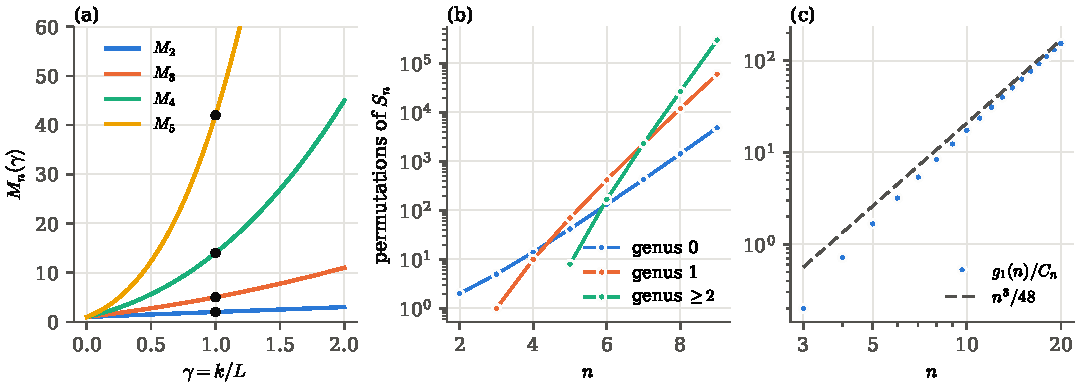
\includegraphics[width=\textwidth]{figures/output/fig03_moments_genus.pdf}
\caption{(a) The genus-zero moments $M_n(\gamma)$ against $\gamma = k/L$; at $\gamma = 1$ they are the Catalan numbers. (b) The permutations of $S_n$ counted by genus relative to $\tau$: genus zero ($C_n$), genus one ($g_1(n)$), and higher. (c) The ratio $g_1(n)/C_n$ and its asymptote $n^3/48$.}
\label{fig03:moments_genus}
\end{figure}

\subsection{The canonical ensemble: the exact planar spectrum}
\label{subsec03:canonical}

In the canonical ensemble the black hole is not in a single fixed-area sector. Following \citet{pssyetal2022} and \citet{wang2023}, the JT density of states and the brane-modified Boltzmann factor are
\begin{equation}
\label{eq03:jt_model}
\rho(E) = \frac{e^{S_0}\sinh\!\big(2\pi\sqrt{2E}\big)}{2\pi^2}, \qquad
y(E) = e^{-\beta E}\; 2^{1-2\mu} \left|\Gamma\!\left(\mu - \tfrac12 + i\sqrt{2E}\right)\right|^2 ,
\end{equation}
where $\mu$ is the brane tension. Put $Z_1 = \int dE\, \rho(E) y(E)$ and
\begin{equation}
\label{eq03:x_and_p}
x(E) = \frac{y(E)}{Z_1}, \qquad p(E) = \rho(E)\, x(E) .
\end{equation}
The black hole sector then has eigenvalues $x(E)$ with density of states $\rho(E)$, and $p(E)$ is the canonical probability density of the energy. Its von Neumann entropy is $S_{\mathrm{BH}} = -\int dE\, p(E) \log x(E)$, and the identity
\begin{equation}
\label{eq03:mixing_identity}
-\!\int dE\, p \log x = \int dE\, p \log \rho \;-\; \int dE\, p \log p
\end{equation}
splits it into the mean microcanonical entropy and the entropy of mixing of the energy distribution.

The exact planar radiation spectrum in this ensemble is determined by the resolvent equation of \citet{pssyetal2022}, exact at planar order (their Eq.~(2.34)), which they solve numerically. \citet{wang2023} observes that the replica sum is combinatorially a free multiplicative convolution of the matter and gravitational spectra, with the gravitational partition functions entering as the free cumulants of a free compound Poisson law. \citet{chengetal2024} reach the same structure from random tensor networks. For the flat matter of the west-coast model, the law $\nu$ of the eigenvalues of $k\rho_{\mathrm{rad}}$ is the free compound Poisson law with $R$-transform
\begin{equation}
\label{eq03:canonical_R}
R(w) = \int dE \; \frac{p(E)}{1 - k\, x(E)\, w} = \mathbb{E}_P\!\left[\frac{1}{1 - a w}\right],
\end{equation}
where $P$ is the law of $a = k\,x(E)$ when $E$ is drawn from $p$. Equivalently, $\nu$ is free compound Poisson with L\'evy measure $a^{-1}P(da)$, and its Cauchy transform $G$ solves
\begin{equation}
\label{eq04:selfconsistent}
G(z) = \frac{1}{z - R\big(G(z)\big)} .
\end{equation}
In random-matrix terms $\nu$ is the limiting spectral law of a Gram matrix whose population spectrum is that of the black hole. At fixed area $P$ is a single atom at $a = \gamma$ and~\eqref{eq03:canonical_R} reduces to~\eqref{eq03:R_transform_scaled}. The entropy of the radiation is
\begin{equation}
\label{eq03:canonical_entropy}
S_{\mathrm{planar}} = \log k - \int u \log u \; d\nu(u),
\end{equation}
by the argument of~\eqref{eq03:svn_from_mp}. Only the law $P$ of the jumps enters: the radiation spectrum depends on the black hole only through its eigenvalue distribution weighted by the canonical probabilities.

\subsection{Relation to prior derivations of the spectrum}
\label{subsec03:positioning}

\citet{pssyetal2022} obtain the same planar content by summing all planar geometries through a Schwinger--Dyson equation for the resolvent of $\rho_{\mathrm{rad}}$, at fixed area and in the canonical ensemble; the resolvent is the Cauchy transform of the spectral law whose moments are computed here. Their Appendix~E counts the planar geometries by Narayana numbers and shows that at planar order the von Neumann entropy of the smaller of two subsystems of a random state, of dimensions $d \le d'$, is exactly $\log d - d/(2d')$. The moment form makes the two-saddle truncation visible moment by moment, through the ratio $C_n/2$, which the resolvent does not display because it keeps all planar diagrams by construction.
 The random-state half of the identification is classical~\citep{lubkin1978, lloydpagels1988, page1993entropy}.

Several recent works approach the same circle of ideas. \citet{liuvardhan2021} derive replica-wormhole entropies for equilibrated pure states through sums over permutations in which non-crossing terms dominate; \citet{urbach2021} treats typical pure states; \citet{jindalhosur2024} develop generalized free cumulants for quantum chaotic systems. \citet{muck2024} identifies the Marchenko--Pastur law in a different gravitational object, the Gram matrix of semiclassical ensembles of black hole microstates. Closest to the transition region, \citet{kudlerflamrath2022} find that subdominant replica-wormhole saddles are enhanced near entanglement transitions; the Catalan ratio of Section~\ref{subsec02:two_saddle} is the same enhancement seen in the R\'enyi moments.

\section{The Diagonal Approximation and the Broadened Page Curve}
\label{sec04:area_fluctuations}

Proposition~\ref{prop03:exact_deficit} describes the transition at fixed area, where the black hole entropy $S_{\mathrm{BH}} = \log L$ is a parameter. In gravity the area of the quantum extremal surface fluctuates, and so does $S_{\mathrm{BH}} = A/4G_N$~\citep{bekenstein1973}. The standard way to include this is the \emph{diagonal approximation} of \citet{marolfwangwang2020}. This section states it, fixes the precise form in which it is compared with the exact planar spectrum in Section~\ref{sec45:exact_correction}, and records the closed form it produces for a Gaussian area distribution.

\subsection{Area fluctuations}
\label{subsec04:fluctuation_mechanism}

\citet{penington2020} observed, in Section~4.4 of that work, that $O(\sqrt{G_N})$ fluctuations in the horizon area and $O(\sqrt{S})$ fluctuations in the energy of the Hawking radiation leave no single well-defined quantum extremal surface near the Page time, and estimated that the transition is smeared over a window of $O(\beta\sqrt{S_{\mathrm{BH}}})$ in time. The phenomenon is not specific to gravity: \citet{vidmarrigol2017} and \citet{murthysrednicki2019} showed that an entanglement transition between nearly equal subsystems acquires a correction set by the square root of the heat capacity in systems obeying the eigenstate thermalization hypothesis.

In JT gravity~\citep{jackiwteitelboim1985, saadetal2019} the canonical partition function is
\begin{equation}
\label{eq04:jt_partition}
Z(\beta) \propto \beta^{-3/2} \exp\left(\frac{2\pi^2}{\beta} + S_0\right),
\end{equation}
and since $\delta S = \beta\, \delta E$ at fixed $\beta$, the variance of the entropy is the heat capacity:
\begin{equation}
\label{eq04:specific_heat}
\sigma^2 = \beta^2\,\langle (\Delta E)^2 \rangle = \beta^2\,\frac{\partial^2}{\partial\beta^2} \log Z = C_V = \frac{4\pi^2}{\beta} + \frac32 ,
\end{equation}
the constant coming from the $\beta^{-3/2}$ prefactor. The Gaussian closed form below uses the leading value $\sigma^2 = 4\pi^2/\beta$, which at $\beta = 2\pi$ gives $\sigma \approx 2.51$; Section~\ref{sec05:exact_jt} uses the exact distribution. The width $\sigma$ is independent of $S_0$ and comparable with the width of order one of the fixed-area transition, so the fluctuations reshape the transition rather than merely shifting it.

\subsection{The diagonal approximation}
\label{subsec04:diagonal}

\citet{marolfwangwang2020} decompose the state into fixed-area states, $|\psi\rangle = \sum_A \sqrt{P(A)}\,|\psi\rangle_A$, so that the radiation density matrix splits into a diagonal part $\sum_A P(A)\rho_R(A)$ and an off-diagonal remainder. Treating the $\rho_R(A)$ as supported on mutually orthogonal subspaces, which they flag as an additional assumption, the entropy of the diagonal part is
\begin{equation}
\label{eq04:diagonal_identity}
S\!\left(\textstyle\sum_A P(A)\rho_R(A)\right) = \sum_A P(A)\, S\big(\rho_R(A)\big) \;-\; \sum_A P(A)\log P(A),
\end{equation}
the second term being the entropy of mixing. Their diagonal approximation keeps the first term: the entropy is the expectation of the fixed-area entropy in the ensemble the state defines (their Eq.~(1.2)). They offer it as a conjecture, supported by consistency with \citet{murthysrednicki2019} and \citet{pssyetal2022}, and bound the neglected entropy of mixing by the logarithm of the number of area values, of order $\log G_N$, which is small compared with the $O(G_N^{-1/2})$ effect they study.

Both terms of~\eqref{eq04:diagonal_identity} depend on how finely the area is resolved: refining the windows lowers each $S(\rho_R(A))$ and raises the entropy of mixing. The dependence cancels, at the order of interest here, in the form we use. Label the black hole eigenvalue levels by their value $x$ and weight each by its canonical probability; in the notation of Section~\ref{subsec03:canonical} the levels are $x(E)$ with weights $p(E)$. Treat each level as a fixed-area black hole of dimension $1/x$, whose radiation entropy is given exactly by Proposition~\ref{prop03:exact_deficit}, and average:
\begin{equation}
\label{eq04:level_resolved}
\boxed{\,S_{\mathrm{diag}} = \int dE\; p(E)\left[\min\!\big(\log k,\, -\log x(E)\big) - \tfrac{1}{2}\, e^{-|\log k + \log x(E)|}\right]}
\end{equation}
This is the diagonal approximation in which each sector's entropy is its contribution $-\log x$ to the black hole's von Neumann entropy, so that the entropy of mixing is carried inside the sector entropies. It has three properties that fix it as the right comparison. It does not depend on any choice of area windows. It reduces to $\log k$ well before the Page time and to the black hole's von Neumann entropy $S_{\mathrm{BH}} = -\int p \log x$ well after it, both of which the exact answer obeys. And it agrees with the diagonal approximation of \citet{marolfwangwang2020} at the order $G_N^{-1/2}$ at which they formulate it, differing from their window-resolved versions only in the bookkeeping of the entropy of mixing, which is $O(\log G_N)$. That bookkeeping is not small at order one. For a Gaussian distribution of width $\sigma$ at the Page point, Eq.~(1.2) of \citet{marolfwangwang2020} evaluated with area windows of width $w$, without the entropy of mixing, lies below the exact planar entropy by $2.37$ nats at $\sigma = 10$, $w = 1$ and by $5.47$ nats at $\sigma = 640$, $w = 0.1$, an amount that grows logarithmically, about as $\tfrac12\log(\sigma/w)$; the right-hand side of~\eqref{eq04:diagonal_identity}, with the full entropy of mixing, lies above it instead (Section~\ref{subsec45:mechanism}). \citet{chengetal2024}, reviewing the holographic argument, make the same point: order-one Marchenko--Pastur effects are irrelevant at the precision of the windowed form, since the entropy of mixing already leads to $O(\log G_N)$ deviations (their Appendix~A.2.2). Statements about the diagonal approximation at order one therefore require a window-free form, and~\eqref{eq04:level_resolved} is the natural one. Its first term is the entropy functional $H_*$ of Section~4 of \citet{chengetal2024}, which under their assumptions reproduces the exact entropy to within $O(\log n)$; \citet{peningtonrath2025} derive the diagonal approximation for R\'enyi entropies, for two extremal surfaces, up to $O(\log G_N)$.


We write $\delta = -\log(k\,x)$ for the signed distance of a level from the radiation, so that $-\log x = \log k + \delta$, and
\begin{equation}
\label{eq04:pssy_entropy}
S_{\mathrm{wc}}(S_{\mathrm{rad}}, S_{\mathrm{BH}}) = \min(S_{\mathrm{rad}}, S_{\mathrm{BH}}) - \frac{1}{2} e^{-|S_{\mathrm{rad}} - S_{\mathrm{BH}}|}
\end{equation}
for the fixed-area entropy with $S_{\mathrm{BH}} = -\log x$. Equation~\eqref{eq04:level_resolved} is then the average of~\eqref{eq04:pssy_entropy} over the distribution of $S_{\mathrm{BH}}$ induced by $p$:
\begin{equation}
\label{eq04:convolution}
S_{\mathrm{diag}}(S_{\mathrm{rad}}) = \int dS_{\mathrm{BH}}\; P(S_{\mathrm{BH}})\; S_{\mathrm{wc}}(S_{\mathrm{rad}}, S_{\mathrm{BH}}) .
\end{equation}

The error of the diagonal approximation is not controlled by the genus expansion. Genus-one effects enter the fixed-area kernel at $O(e^{-2S_0})$ (Section~\ref{subsec03:genus_one}); the diagonal approximation is a statement within the planar sector, about replacing the entropy of a superposition of sectors by an average over sectors, and its error is a planar effect. Because the exact planar answer is known in this model (Section~\ref{subsec03:canonical}), that error can be computed, and Section~\ref{sec45:exact_correction} computes it.

\subsection{Gaussian broadening: the closed form}
\label{subsec04:gaussian_broadening}

For a Gaussian distribution of the black hole entropy,
\begin{equation}
\label{eq04:gaussian_dist}
P(S_{\mathrm{BH}}) = \frac{1}{\sqrt{2\pi}\sigma} \exp\left(-\frac{(S_{\mathrm{BH}} - \langle S_{\mathrm{BH}}\rangle)^2}{2\sigma^2}\right),
\end{equation}
the average~\eqref{eq04:convolution} splits into two elementary integrals, one for each term of~\eqref{eq04:pssy_entropy} (Appendix~\ref{app:broadening_integrals}). Write $\Phi$ and $\phi$ for the standard normal distribution function and density, and $\Delta = S_{\mathrm{rad}} - \langle S_{\mathrm{BH}}\rangle$. The minimum averages to\footnote{Up to sign and constants, this Gaussian expectation of a minimum coincides with the classical price formula for a put option in the arithmetic-Brownian-motion model of \citet{bachelier1900}; beyond this identity of integrals, nothing from that setting enters the derivation.}
\begin{equation}
\label{eq04:E_min_alt}
E_{\min}(\Delta, \sigma) = \langle S_{\mathrm{BH}}\rangle + \Delta\, \Phi\!\left(-\frac{\Delta}{\sigma}\right) - \sigma\, \phi\!\left(\frac{\Delta}{\sigma}\right),
\end{equation}
and the fixed-area correction to
\begin{equation}
\label{eq04:E_corr}
E_{\mathrm{corr}}(\Delta, \sigma) = -\frac{1}{2} e^{\sigma^2/2} \left[ e^{-\Delta} \Phi\!\left(\frac{\Delta - \sigma^2}{\sigma}\right) + e^{\Delta} \Phi\!\left(\frac{-\Delta - \sigma^2}{\sigma}\right) \right],
\end{equation}
the factor $e^{\sigma^2/2}$ arising from the Gaussian moment generating function. The diagonal approximation is then
\begin{equation}
\label{eq04:S_grav}
S_{\mathrm{diag}}(\Delta, \sigma) = E_{\min}(\Delta, \sigma) + E_{\mathrm{corr}}(\Delta, \sigma),
\end{equation}
and we write $\mathcal{F}_\sigma(\Delta) = S_{\mathrm{diag}} - \min(S_{\mathrm{rad}}, \langle S_{\mathrm{BH}}\rangle)$ for its deficit.

$E_{\min}$ is Eq.~(3.14) of \citet{marolfwangwang2020} in different notation. Their crossover function, in the notation of \citet{murthysrednicki2019}, is $\Phi_{\mathrm{MS}}(x) = e^{-x^2} + \sqrt{\pi}\,|x|\,(\mathrm{erf}\,|x| - 1)$, and
\begin{equation}
\label{eq04:ms_bridge}
\Phi_{\mathrm{MS}}\big(u/\sqrt2\big) = \sqrt{2\pi}\,\big[\phi(u) - |u|\,\Phi(-|u|)\big],
\end{equation}
so that their $-\big(\sigma/\sqrt{2\pi}\big)\Phi_{\mathrm{MS}}\big(\Delta/(\sigma\sqrt2)\big)$ is $\mathcal{F}_\sigma(\Delta)$ without the $E_{\mathrm{corr}}$ term. The same leading behaviour is in \citet{pssyetal2022}: in the canonical ensemble at the Page point, for $\mu \gg 1/\beta$, they find $S = \log k - \sqrt{2\pi/\beta} + O(1)$, which is $-\sigma/\sqrt{2\pi}$ with $\sigma^2 = 4\pi^2/\beta$.

The $E_{\mathrm{corr}}$ term is what the diagonal approximation produces when the exact fixed-area kernel, rather than the minimum alone, is averaged. At the Page point it decays as $|E_{\mathrm{corr}}(0,\sigma)| \simeq 1/(\sigma\sqrt{2\pi})$. Section~\ref{sec45:exact_correction} shows that the exact planar answer differs from~\eqref{eq04:S_grav} by an amount that tends to a constant, and that its own $1/\sigma$ term has a different coefficient. The $E_{\mathrm{corr}}$ term is therefore a property of the approximation, not of the broadened Page curve, and we keep it in the closed form only for completeness.

\subsection{Properties of the broadened curve}
\label{subsec04:properties}

\paragraph{Peak deficit.} At the Page time,
\begin{equation}
\label{eq04:peak_deficit}
\mathcal{F}_\sigma(0) = -\frac{\sigma}{\sqrt{2\pi}} - e^{\sigma^2/2}\,\Phi(-\sigma),
\end{equation}
which tends to $-\tfrac12$ as $\sigma \to 0$, recovering the fixed-area value, and to $-\sigma/\sqrt{2\pi}$ as $\sigma \to \infty$. The two terms are equal at $\sigma \approx 0.75$; above it the broadened minimum dominates and the fixed-area correction is an algebraically decaying perturbation.

\paragraph{Width.} The deficit is appreciable over a range of $\Delta$ of order $\sigma$. With $\Delta \sim \delta t/\beta$, the window in time is
\begin{equation}
\label{eq04:width_time_general}
\delta t \;\sim\; \beta\,\sigma \;=\; \beta\,\sqrt{C_V} .
\end{equation}
In JT gravity at fixed $\beta$, $C_V = 4\pi^2/\beta$ is independent of $S_0$ and the window is $O(\beta)$. For black holes whose heat capacity grows with their entropy, as for large AdS--Schwarzschild black holes, $\sigma \sim \sqrt{S_{\mathrm{BH}}}$ and
\begin{equation}
\label{eq04:width_time_highD}
\delta t \;\sim\; \beta\,\sqrt{S_{\mathrm{BH}}},
\end{equation}
which agrees with Penington's estimate.

\paragraph{Rescaled form.} With $u = \Delta/\sigma$,
\begin{equation}
\label{eq04:universal}
\frac{\mathcal{F}_\sigma(\Delta)}{\sigma} \;\xrightarrow{\;\sigma \to \infty\;}\; -\big[\phi(u) - |u|\,\Phi(-|u|)\big],
\end{equation}
a single curve with peak $-1/\sqrt{2\pi}$ at $u = 0$ and tails falling as $\phi(u)/u^2$. Figure~\ref{fig04:broadened} shows the deficit for several $\sigma$ and the collapse onto~\eqref{eq04:universal}.

\begin{figure}[htbp]
\centering
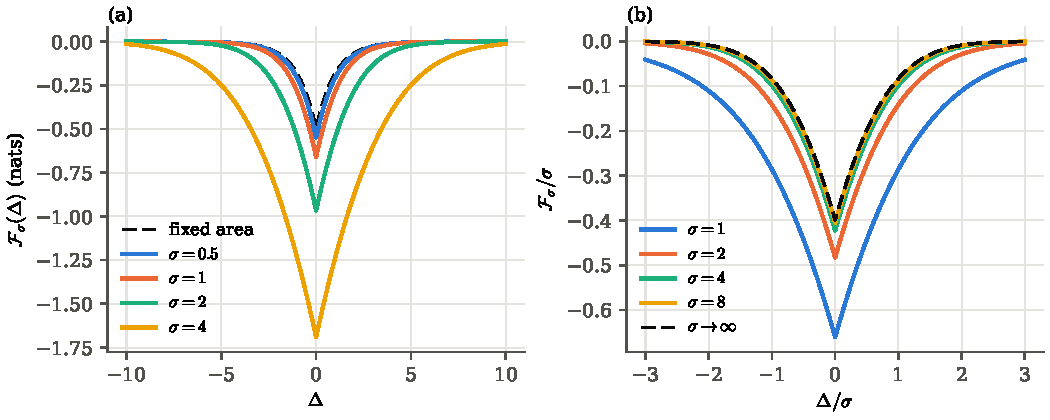
\includegraphics[width=\textwidth]{figures/output/fig04_broadened.pdf}
\caption{The diagonal approximation for a Gaussian area distribution. (a) The deficit $\mathcal{F}_\sigma(\Delta)$ for $\sigma = 0$ (fixed area), $0.5$, $1$, $2$ and $4$. (b) The same curves rescaled, $\mathcal{F}_\sigma/\sigma$ against $\Delta/\sigma$, approaching the limit~\eqref{eq04:universal} (dashed) as $\sigma$ grows.}
\label{fig04:broadened}
\end{figure}

\subsection{Dependence on the fluctuation width}
\label{subsec04:sensitivity}

The closed form gives the response of the curve to the heat capacity directly. Differentiating~\eqref{eq04:E_min_alt} with $\phi'(z) = -z\phi(z)$,
\begin{equation}
\label{eq04:dsigma_min}
\frac{\partial E_{\min}}{\partial \sigma} = -\phi\!\left(\frac{\Delta}{\sigma}\right),
\end{equation}
and differentiating~\eqref{eq04:E_corr}, with the identity $e^{\sigma^2/2}e^{\mp\Delta}\,\phi\big((\pm\Delta-\sigma^2)/\sigma\big) = \phi(\Delta/\sigma)$,
\begin{equation}
\label{eq04:dsigma_corr}
\frac{\partial E_{\mathrm{corr}}}{\partial \sigma} = \sigma\,E_{\mathrm{corr}} + \phi\!\left(\frac{\Delta}{\sigma}\right).
\end{equation}
The two $\phi(\Delta/\sigma)$ terms cancel, leaving
\begin{equation}
\label{eq04:dsigma_total}
\frac{\partial S_{\mathrm{diag}}}{\partial \sigma} = \sigma\,E_{\mathrm{corr}}(\Delta,\sigma) \;\le\; 0,
\end{equation}
which at the Page time is $-\sigma e^{\sigma^2/2}\Phi(-\sigma)$, rising in magnitude from $0$ at $\sigma = 0$ to $1/\sqrt{2\pi}$ as $\sigma \to \infty$. Within the diagonal approximation, larger area fluctuations always deepen the deficit.

\section{The Exact Correction to the Diagonal Approximation}
\label{sec45:exact_correction}

This section compares the exact planar entropy $S_{\mathrm{planar}}$ of Section~\ref{subsec03:canonical} with the diagonal approximation $S_{\mathrm{diag}}$ of~\eqref{eq04:level_resolved}. Both are determined by a single probability law. Let $P$ be the law of $a = k\,x$ when the black hole level $x$ is drawn with its canonical weight, and put
\begin{equation}
\label{eq45:delta}
\delta = -\log a = -\log(k\,x), \qquad q = P(\delta > 0) = P\big(-\log x > \log k\big).
\end{equation}
A level with $\delta > 0$ is larger than the radiation, in the sense that a fixed-area black hole of dimension $1/x$ would exceed $k$; the number $q$ is the canonical weight of such levels, and it falls from one to zero as the radiation grows. It is close to the pre-Page probability of \citet{akersetal2022}, the weight $1 - p_k$ of the black hole spectrum beyond its $k$ largest eigenvalues in the notation of \citet{pssyetal2022}, and the two coincide in the broad-distribution limit, but slowly: they differ by an amount of order $\log\sigma/\sigma$, and for a Gaussian law at the Page point the pre-Page probability is $0.37$ at $\sigma = 10$ and $0.48$ at $\sigma = 100$, against $q = \tfrac12$. At the Page point, where $\log k$ equals the mean of $-\log x$, $q$ is the probability that $-\log x$ exceeds its mean. It tends to $\tfrac12$ when the median and the mean of $-\log x$ differ by $o(\sigma)$, as for symmetric laws and for the JT law of Section~\ref{sec05:exact_jt}, but not for laws whose skewness persists as they broaden.

The result is that the difference between the two entropies tends to $-q\log q$ when the area distribution is broad on the scale of one nat, and so to $\tfrac12\log 2$ at the Page point when $q$ tends to $\tfrac12$ there. Section~\ref{subsec45:representation} reduces $S_{\mathrm{planar}}$ to a one-dimensional integral; Section~\ref{subsec45:theorem} proves the limit; Section~\ref{subsec45:mechanism} explains it and relates it to earlier work; Section~\ref{subsec45:first_order} gives the first correction; Section~\ref{subsec45:consequences} draws the consequences.

\subsection{A one-dimensional representation}
\label{subsec45:representation}

The exact spectrum is defined by the fixed point~\eqref{eq04:selfconsistent}. On the negative real axis that fixed point can be solved explicitly for the spectral parameter, which removes both the fixed-point iteration and the Stieltjes inversion.

\begin{proposition}[Representation]
\label{thm45:representation}
Let $P$ be a probability law on $(0,\infty)$ with $\mathbb{E}_P[a] < \infty$, let $\nu$ be the free compound Poisson law with $R$-transform $R(w) = \mathbb{E}_P[(1 - a w)^{-1}]$, and define
\begin{equation}
\label{eq45:h_s}
h(v) = \mathbb{E}_P\!\left[\frac{1}{1 + a\, e^{v}}\right], \qquad s(v) = e^{-v} - h(v),
\end{equation}
with $v_0 \in [0,\infty]$ the first zero of $s$ on $[0,\infty)$, and
\begin{equation}
\label{eq45:J}
J(v) = \frac{\big(1 - h\big)\big(1 - h\, e^{v}\big)\big(1 + h'\, e^{v}\big)}{1 + (1 - h)\, e^{v}} .
\end{equation}
Then
\begin{equation}
\label{eq45:FA}
\int u \log u\; d\nu(u) = \int_{-\infty}^{v_0} J(v)\, dv ,
\end{equation}
and
\begin{equation}
\label{eq45:gap_exact}
S_{\mathrm{planar}} - S_{\mathrm{diag}} = -\int_{-\infty}^{v_0} \Big[ J(v) - \big(1 - h(v)\big)\mathbb{1}_{v<0} \Big] dv \;-\; \mathbb{E}\big[\log(1 + e^{-|\delta|})\big] \;+\; \tfrac12\, \mathbb{E}\big[e^{-|\delta|}\big] .
\end{equation}
\end{proposition}

The proof is in Appendix~\ref{app:proofs}. Its content is that $e^{v} = \int d\nu(u)/(u + s)$ inverts to the explicit curve $s(v)$, so that the identity $\int u\log u\, d\nu = \int_0^\infty [\,1/(1+s) - 1 + s\, e^{v(s)}]\, ds$ becomes an integral in $v$; subtracting $\int_{-\infty}^0 (1-h)\, dv = \mathbb{E}[\log(1 + e^{-\delta})]$ removes the part of the integrand that grows with the width of $P$. The integrand of~\eqref{eq45:gap_exact} is bounded by $\tfrac54 e^{v}$ for $v < 0$ and by $1$ on $[0, v_0)$, so the gap is a single quadrature over an interval whose length does not depend on the width of $P$. At fixed area, $P$ is one atom and~\eqref{eq45:FA} reproduces Proposition~\ref{prop03:exact_deficit} to machine precision.

\subsection{The broad-distribution limit}
\label{subsec45:theorem}

\begin{theorem}
\label{thm45:limit}
Let $(P_n)$ be jump laws with $\mathbb{E}_{P_n}[a] < \infty$ such that, for every $M > 0$,
\begin{equation}
\label{eq45:spreading}
P_n\big(|\delta| \le M\big) \to 0 ,
\end{equation}
and $q_n = P_n(\delta > 0) \to q \in (0,1)$. Then
\begin{equation}
\label{eq45:limit}
\boxed{\;S_{\mathrm{planar}} - S_{\mathrm{diag}} \;\longrightarrow\; -\,q \log q \;}
\end{equation}
\end{theorem}

The condition~\eqref{eq45:spreading} says that the area distribution becomes broad compared with one nat around the radiation entropy, so that no finite fraction of the canonical weight stays near the transition. It cannot be dropped: if a fixed fraction of the weight remains at $|\delta| = O(1)$, the limit is different (Appendix~\ref{app:proofs}).

The proof (Appendix~\ref{app:proofs}) uses only~\eqref{eq45:gap_exact}. Under~\eqref{eq45:spreading} the two expectations vanish, $h$ tends to $q$ uniformly on compact sets, $h'$ tends to zero, and $v_0$ tends to $-\log q$. Dominated convergence then reduces the integral to that of the limiting integrand
\begin{equation}
\label{eq45:J_limit}
J_\infty(v) - (1-q)\mathbb{1}_{v<0} =
\begin{cases}
-\dfrac{(1-q)\, e^{v}}{1 + (1-q)\, e^{v}}, & v < 0, \\[2.2ex]
\dfrac{1}{1 + (1-q)\, e^{v}} - q, & 0 \le v < -\log q ,
\end{cases}
\end{equation}
whose two pieces integrate to $-\log(2-q)$ and $\log(2-q) + q\log q$.

\begin{corollary}
\label{thm45:gaussian}
If $-\log x$ is normally distributed with mean $\langle S_{\mathrm{BH}}\rangle$ and variance $\sigma^2$, and $\Delta = \log k - \langle S_{\mathrm{BH}}\rangle$, then as $\sigma \to \infty$ with $\Delta/\sigma \to \theta$,
\begin{equation}
S_{\mathrm{planar}} - S_{\mathrm{diag}} \to -q\log q, \qquad q = \Phi(-\theta) .
\end{equation}
At the Page point the limit is $\tfrac12\log 2 \approx 0.3466$ nats. Over all $\theta$ it is largest, equal to $1/e$, at $q = 1/e$, that is $\theta = \Phi^{-1}(1 - 1/e) \approx 0.337$, after the Page time.
\end{corollary}

In the JT model the width is $\sigma^2 = C_V = 4\pi^2/\beta + \tfrac32$, so the limit is approached at high temperature; Section~\ref{sec05:exact_jt} shows that it is. The theorem does not assume a Gaussian law: it holds for any family that spreads in the sense of~\eqref{eq45:spreading}, and we have checked it numerically for uniform, skew-normal and two-sector families (Appendix~\ref{app:numerical}). The shape of the law enters the limit only through $q$, but that includes the value at the Page point: for a skew-normal law of shape parameter $4$, with $\log k$ at its mean, $q$ tends to $0.439$ and the limit is $0.361$ rather than $\tfrac12\log 2$. The theorem is a statement about the free compound Poisson law of Section~\ref{subsec03:canonical}, and it applies to the radiation of any model whose planar spectrum takes that form; Section~\ref{subsec06:meaning} discusses which models these are.

\subsection{Mechanism, and relation to earlier work}
\label{subsec45:mechanism}

The limit has a transparent origin, which the simplest case exposes. Let the black hole have two groups of levels: weight $q$ on levels far larger than the radiation, $\delta \gg 1$, and weight $1-q$ on levels far smaller, $\delta \ll -1$. The levels of the first group number far more than $k$; their contributions to $\rho_{\mathrm{rad}}$ are random rank-one terms on the same $k$-dimensional space, and together they average to a multiple of the identity, a flat floor $q\,\mathbb{1}_k/k$ under the spectrum. The levels of the second group occupy nearly orthogonal subspaces of the radiation and sit on top of that floor. The entropy is then
\begin{equation}
\label{eq45:two_sector}
S_{\mathrm{planar}} \simeq \underbrace{q\log k - q\log q}_{\text{floor}} \;+\; \underbrace{(1-q)\,\mathbb{E}\big[-\log x \,\big|\, \delta < 0\big] + \dots}_{\text{levels below } 1/k}\,,
\end{equation}
where the second term is $-\sum x\log x$ over the levels of the second group, whose eigenvalues are their canonical weights $x$, so that the entropy of mixing among them is already included. The diagonal approximation assigns $\log k$ to each level of the first group, for $q\log k$ in total, and to the second group the same entropy, through the sector entropy $-\log x$. The difference is $-q\log q$, exactly: the radiation resolves the levels smaller than itself but not those larger, so the entropy of mixing among the larger ones collapses into the single block term $-q\log q$. Numerically the two-group model reproduces $-q\log q$ to six digits once the groups are separated by $e^{16}$ (Appendix~\ref{app:numerical}). Theorem~\ref{thm45:limit} says that a broad distribution behaves in the same way, because the levels within $O(1)$ of the radiation, the only ones whose contribution is neither of these two, carry vanishing weight.

The mechanism is not new, and the constant is implicit in earlier work. \citet{pssyetal2022} identify the flat floor in the canonical ensemble: they write the radiation density matrix as the black hole density matrix projected onto its $k$ largest eigenvalues, plus a multiple $(1 - p_k)/k$ of the identity that collects the remaining states of the spectrum. Their shifted thermal spectrum (their Eq.~(F.56)), which they estimate to be accurate to $O(\beta)$, contains this block, whose contribution to the entropy, $-(1 - p_k)\log\big((1-p_k)/k\big)$, they write out in their discussion of that equation; and they note that their approximate entropy agrees with the average of the microcanonical answer to within $O(1)$. They do not evaluate that difference: their Page-point result $S = \log k - \sqrt{2\pi/\beta} + O(1)$, obtained from a cruder approximation at a single value of $k$, leaves it inside the remainder. The shifted thermal spectrum is in fact more accurate than an order-one statement: for Gaussian laws at the Page point it differs from the exact planar entropy by $0.025$ nats at $\sigma = 10$ and by $1.8\times10^{-4}$ nats at $\sigma = 200$, well below the first correction $K/\sigma$ of Section~\ref{subsec45:first_order}, so both the constant and the first correction are implicit in it. \citet{akerspenington2021} treat a black hole whose bulk state is a mixture of two components at fixed area (their Section~4.3, with details in their Appendix~A); in the regime where one component has crossed the transition and the other has not, their entropy contains the block term of~\eqref{eq45:two_sector}, and in the regime where both have crossed they note that the Shannon term is absent. What the present section adds is their evaluation, the identification of the constant as the limit of the error of the diagonal approximation for every spreading family, and a proof from the exact planar spectrum rather than from an approximation to it. For random tensor networks with two competing minimal cuts and continuous link spectra, \citet{chengetal2024} show that the entropy is $H_*$, the first term of~\eqref{eq04:level_resolved}, up to $O(\log n)$; \citet{peningtonrath2025} derive the diagonal approximation for holographic R\'enyi entropies up to $O(\log G_N)$. In the present setting the theorem determines the remainder at order one.

\citet{marolfwangwang2020} anticipate where the orthogonality assumption behind~\eqref{eq04:diagonal_identity} can fail. The density matrices of their sectors are orthogonal for different values of the area $A_1$ of the surface nearer the region, but, they note, ``the same need not always hold for $A_2$ since it can be reconstructed on $R$ only for $A_2 < A_1$'' (their Section~3.2). For the radiation of the west-coast model $A_1/4G_N$ corresponds to $\log k$ and $A_2/4G_N$ to the entropy of the black hole, so the sectors that need not be orthogonal are those larger than the radiation, up to the difference $-\log p$ between the area and the sector entropy $-\log x$ of~\eqref{eq03:mixing_identity}, which moves the boundary by an amount of order $\log\sigma$. They treat all sectors as orthogonal, as an additional assumption. The theorem measures the cost: sectors smaller than the radiation are supported on nearly orthogonal subspaces of it, and for them the assumption holds; sectors larger than the radiation all fill the same space, and the entropy of mixing among them, which the assumption counts in full, collapses to the block term. Write $S_D$ for the right-hand side of~\eqref{eq04:diagonal_identity} with area windows of any fixed width, and $H(P\,|\,\mathrm{large})$ for the entropy of mixing among the windows larger than the radiation, which carry total weight $q'$. Then
\begin{equation}
\label{eq45:mww_form}
S_{\mathrm{planar}} = S_D - q'\, H(P\,|\,\mathrm{large}) + o(1)
\end{equation}
for laws with a smooth density of width $\sigma$. The argument, in Appendix~\ref{subsecD:windows}, is heuristic, and we state~\eqref{eq45:mww_form} on the strength of it and of the numerics: for Gaussian laws at the Page point and windows of unit width, $S_D - q' H(P\,|\,\mathrm{large}) - S_{\mathrm{planar}}$ is $0.305$, $0.124$, $0.044$ and $0.020$ at $\sigma = 10$, $40$, $160$ and $640$. The window dependence of $S_D$ and of the subtracted term cancel, but the approach is slow, with corrections of order $(\log\sigma)^2/\sigma$; the level-resolved form~\eqref{eq04:level_resolved} avoids windows altogether and converges as $1/\sigma$.

\subsection{The first correction}
\label{subsec45:first_order}

When $\delta$ has a smooth density, the approach to the limit can be computed. Let $f$ be the density of $\delta$, and suppose that near $\delta = 0$ it is of order $1/\sigma$ and varies on the scale $\sigma$: $f(0) = O(\sigma^{-1})$ and $f' = O(\sigma^{-2})$. Expanding~\eqref{eq45:gap_exact} to first order in $1/\sigma$ at fixed $q$ gives (Appendix~\ref{subsecD:first_order})
\begin{equation}
\label{eq45:first_order_general}
S_{\mathrm{planar}} - S_{\mathrm{diag}} = -q\log q \;-\; f(0)\left(\frac{\pi^2}{6} + \log q + \frac12 \log^2 q\right) + O(\sigma^{-2}).
\end{equation}
For a Gaussian law of width $\sigma$, with $\theta = \Delta/\sigma$, $q = \Phi(-\theta)$ and $f(0) = \phi(\theta)/\sigma$, this reads
\begin{equation}
\label{eq45:first_order}
S_{\mathrm{planar}} - S_{\mathrm{diag}} = -q\log q \;-\; \frac{\phi(\theta)}{\sigma}\left(\frac{\pi^2}{6} + \log q + \frac12 \log^2 q\right) + O(\sigma^{-2}),
\end{equation}
and at the Page point
\begin{equation}
\label{eq45:first_order_page}
S_{\mathrm{planar}} - S_{\mathrm{diag}} = \frac12\log 2 - \frac{K}{\sigma} + O(\sigma^{-2}), \qquad K = \frac{\pi^2/6 - \log 2 + \tfrac12\log^2 2}{\sqrt{2\pi}} \approx 0.4755 .
\end{equation}
The derivation controls the remainder only formally, and we state~\eqref{eq45:first_order_general} as an expansion confirmed numerically rather than as a theorem. For Gaussian laws the confirmation is close: at the Page point $\sigma\,[\tfrac12\log 2 - (S_{\mathrm{planar}} - S_{\mathrm{diag}})]$ is $0.4772$, $0.4764$ and $0.4760$ at $\sigma = 100$, $200$ and $400$, extrapolating to $0.4756$; away from it, at $\sigma = 400$, the formula predicts the departure from $-q\log q$ to within $0.6\%$ for every $\theta$ in $[-1.5, 1.5]$ (Table~\ref{tab45:gaussian}). The remainder multiplied by $\sigma^2$ settles near $-0.17$ at the Page point, with no sign of a $\log\sigma$ term. For the skewed JT law, with $f(0)$ read off the exact distribution, the formula predicts the departure to within $1.5\%$ at $\beta = \tfrac1{25}$ (Section~\ref{subsec05:exact_page_curve}).

Combined with the expansion $S_{\mathrm{diag}} - \log k = -\sigma/\sqrt{2\pi} - 1/(\sigma\sqrt{2\pi}) + O(\sigma^{-3})$ of~\eqref{eq04:peak_deficit}, the exact planar deficit at the Page point is
\begin{equation}
\label{eq45:planar_page}
S_{\mathrm{planar}} - \log k = -\frac{\sigma}{\sqrt{2\pi}} + \frac12\log 2 - \frac{1 + \pi^2/6 - \log 2 + \tfrac12\log^2 2}{\sigma\sqrt{2\pi}} + O(\sigma^{-2}) .
\end{equation}
The diagonal approximation reproduces the leading term, the $\sqrt{C/2\pi}$ of \citet{murthysrednicki2019}; it misses the constant $\tfrac12\log 2$; and its own $1/\sigma$ term, $E_{\mathrm{corr}}$, has coefficient $1$ where the exact coefficient is $1 + \pi^2/6 - \log 2 + \tfrac12\log^2 2 \approx 2.19$.

\begin{table}[htbp]
\centering
\caption{Gaussian area distributions: the gap $S_{\mathrm{planar}} - S_{\mathrm{diag}}$ computed from~\eqref{eq45:gap_exact}, against the limit $-q\log q$ and the first-order formula~\eqref{eq45:first_order}. Upper block: the Page point, for several widths. Lower block: $\sigma = 400$ at several $\theta = \Delta/\sigma$. All values in nats.}
\label{tab45:gaussian}
\begin{tabular}{cccccc}
\toprule
$\sigma$ & $\theta$ & $q$ & $S_{\mathrm{planar}} - S_{\mathrm{diag}}$ & $-q\log q$ & first order \\
\midrule
$2.507$ & $0$ & $0.5$ & $0.17877$ & $0.34657$ & $0.15686$ \\
$6.283$ & $0$ & $0.5$ & $0.27039$ & $0.34657$ & $0.27089$ \\
$8.886$ & $0$ & $0.5$ & $0.29224$ & $0.34657$ & $0.29306$ \\
$20$ & $0$ & $0.5$ & $0.32248$ & $0.34657$ & $0.32280$ \\
$100$ & $0$ & $0.5$ & $0.34180$ & $0.34657$ & $0.34182$ \\
\midrule
$400$ & $-1.5$ & $0.93319$ & $0.06402$ & $0.06452$ & $0.06401$ \\
$400$ & $-0.8$ & $0.78814$ & $0.18660$ & $0.18764$ & $0.18660$ \\
$400$ & $0$ & $0.5$ & $0.34538$ & $0.34657$ & $0.34538$ \\
$400$ & $0.337$ & $0.36806$ & $0.36680$ & $0.36788$ & $0.36680$ \\
$400$ & $0.8$ & $0.21186$ & $0.32783$ & $0.32877$ & $0.32783$ \\
$400$ & $1.5$ & $0.06681$ & $0.17994$ & $0.18078$ & $0.17993$ \\
\bottomrule
\end{tabular}
\end{table}

\subsection{Consequences}
\label{subsec45:consequences}

\paragraph{The error is additive.} The diagonal approximation is accurate to a constant, not to a fixed fraction. Relative to the deficit, of order $\sigma$, its error vanishes as $\sigma \to \infty$, and for a macroscopic black hole, with $\sigma \sim \sqrt{S_{\mathrm{BH}}}$, the diagonal approximation is relatively exact. At the widths of the JT model at moderate temperature the constant is not small: at $\beta = 2\pi$ the gap is $16\%$ of the deficit (Section~\ref{sec05:exact_jt}).

\paragraph{The broadened curve is not symmetric.} For a Gaussian area distribution the diagonal approximation is even in $\Delta$. The exact curve is not: the correction $-q\log q$ is largest after the Page time, at $q = 1/e$, and it vanishes like $1 - q$ on the early side, where $q \to 1$, but only like $q\log(1/q)$ on the late side, where $q \to 0$. Figure~\ref{fig45:gap}(a) shows the correction in the JT model at three temperatures, where it is asymmetric in the same way; there the diagonal approximation is itself slightly asymmetric, because the JT law is skewed (Section~\ref{subsec05:three_layer}).

\paragraph{A corrected prescription.} Adding the limit and the first correction to the diagonal approximation,
\begin{equation}
\label{eq45:corrected}
S \;\approx\; S_{\mathrm{diag}} - q\log q - f(0)\left(\frac{\pi^2}{6} + \log q + \frac12 \log^2 q\right),
\end{equation}
reproduces the exact planar entropy at the Page point to $0.02$ nats at $\sigma = 2.5$ and to $5\times10^{-4}$ nats at $\sigma = 6.3$ for Gaussian laws; the limit term alone leaves an error of $0.17$ and $0.08$ nats at the same widths.

\paragraph{The fixed-area correction is not a prediction.} Within the diagonal approximation the fixed-area kernel contributes $E_{\mathrm{corr}} \simeq -1/(\sigma\sqrt{2\pi})$ at the Page point. Equation~\eqref{eq45:planar_page} shows that the true $1/\sigma$ term is larger by a factor of about $2.19$, and that both lie below the constant $\tfrac12\log 2$ once $\sigma \gtrsim 2.5$. The structure of the diagonal approximation below order one should not be read as structure of the Page curve.

\begin{figure}[htbp]
\centering
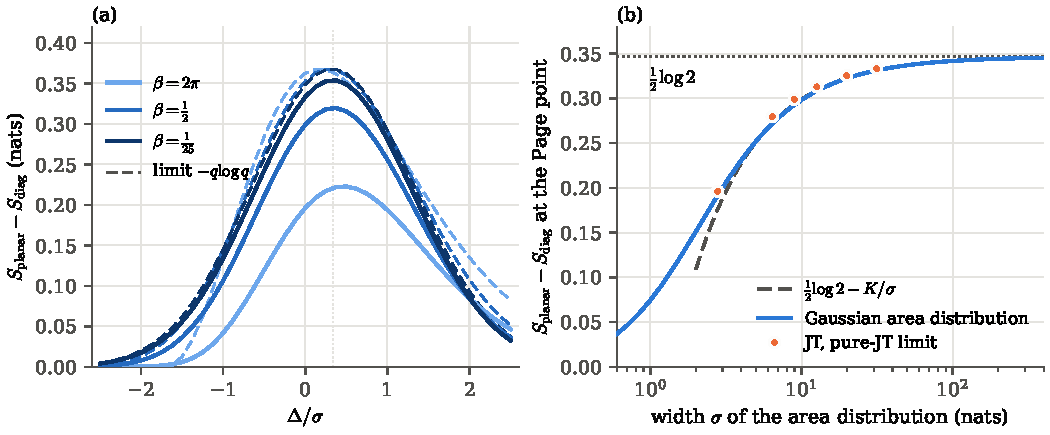
\includegraphics[width=\textwidth]{figures/output/fig45_gap.pdf}
\caption{The exact correction to the diagonal approximation. (a) $S_{\mathrm{planar}} - S_{\mathrm{diag}}$ against $\Delta/\sigma$ for the pure-JT area distribution at $\beta = 2\pi$, $\tfrac12$ and $\tfrac{1}{25}$ (solid), with the broad-distribution limit $-q\log q$ of the same law, $q$ being the JT weight of the levels larger than the radiation (dashed, same colour). The vertical dotted line marks $\Delta/\sigma = \Phi^{-1}(1 - 1/e) \approx 0.337$, where the limit is largest for a Gaussian law.
 (b) The gap at the Page point against the width $\sigma$: Gaussian area distributions (line), the pure-JT model (points), the first-order formula~\eqref{eq45:first_order_page} (dashed) and the limit $\tfrac12\log 2$ (dotted).}
\label{fig45:gap}
\end{figure}

\section{The JT Model}
\label{sec05:exact_jt}

This section applies the results of Section~\ref{sec45:exact_correction} to the area distribution of the west-coast model itself. It states the condition on the brane tension under which that distribution is the JT one, gives the exact correction at several temperatures, separates it from the effect of the non-Gaussian shape of the distribution, and records the R\'enyi entropies through the transition at fixed area.

\subsection{The area distribution}
\label{subsec05:entropy_distribution}

With the density of states and the brane-modified Boltzmann factor of~\eqref{eq03:jt_model}, the canonical weight of the black hole levels is $p(E) = \rho(E)y(E)/Z_1$, and the entropy assigned to a level by the diagonal approximation~\eqref{eq04:level_resolved} is $-\log x(E) = -\log y(E) + \log Z_1$. In the pure JT case, where $y(E) = e^{-\beta E}$, this is $\beta E + \log Z_1$. Its mean is the black hole's von Neumann entropy and its variance is exactly the heat capacity,
\begin{equation}
\label{eq05:sigma_eff}
\mathrm{Var}\big(-\log x\big) = \beta^2\,\mathrm{Var}(E) = C_V = \frac{4\pi^2}{\beta} + \frac32 ,
\end{equation}
the constant coming from the $\beta^{-3/2}$ prefactor of~\eqref{eq04:jt_partition}. The distribution is skewed to the right, with skewness $0.77$, $1.01$ and $1.24$ at $\beta = \pi$, $2\pi$ and $4\pi$, falling to zero as $\beta \to 0$, where it becomes Gaussian. The sector entropy $-\log x$ differs from the microcanonical entropy $S_0 + 2\pi\sqrt{2E}$, the area variable of \citet{marolfwangwang2020}, by $-\log p(E)$, as in~\eqref{eq03:mixing_identity}; the microcanonical entropy is much closer to Gaussian, with skewness $0.05$, $0.13$ and $0.26$ at the same temperatures.

\subsubsection*{The brane-tension condition}

The pure-JT weight requires the brane factor in~\eqref{eq03:jt_model} to act as a constant over the canonical window, where $\sqrt{2E} \approx 2\pi/\beta$. For $\sqrt{2E} \gg \mu$ the factor $|\Gamma(\mu - \tfrac12 + i\sqrt{2E})|^2$ decays as $e^{-\pi\sqrt{2E}}$, which halves the coefficient of $\sqrt{2E}$ in the exponent of $\rho(E)y(E)$, and with it the mean entropy above extremality, from $4\pi^2/\beta$ to $2\pi^2/\beta$. For $\sqrt{2E} \ll \mu$ it is, up to a constant, $e^{-2E\psi'(\mu - 1/2)} \approx e^{-2E/\mu}$, with $\psi'$ the trigamma function, so it shifts the inverse temperature from $\beta$ to about $\beta + 2/\mu$. The JT form of the area distribution therefore requires the large-tension regime
\begin{equation}
\label{eq05:mu_condition}
\mu \gg 2\pi/\beta ,
\end{equation}
which is, up to the factor $2\pi$, the condition $\mu \gg 1/\beta$ assumed by \citet{pssyetal2022} in their Appendix~F; its pure-JT parameters require in addition that the shift be negligible. Since the shift changes the width by about $\sigma/(\beta\mu)$, quantities of order one at the Page point require $\sigma/(\beta\mu) \ll 1$. At $\beta = 2\pi$ the mean of $2\pi\sqrt{2E}$ runs from $3.87$ at $\mu = 0.6$ to $7.27$ at $\mu = 200$, against $2\pi^2/\beta = 3.14$ and $4\pi^2/\beta = 6.28$, while its standard deviation moves only from $2.05$ to $2.30$. All results below are for the pure-JT distribution, the limit $\mu \to \infty$. The exact planar entropy depends on $\mu$ more strongly than its difference from the diagonal approximation: at $\beta = 1$ and the Page point, lowering $\mu$ from $\infty$ to $20$ reduces $\sigma$ from $6.40$ to $6.13$ and moves $S_{\mathrm{planar}} - \log k$ from $-2.33$ to $-2.22$, while the gap moves only from $0.280$ to $0.277$.

\subsection{The exact correction in the JT model}
\label{subsec05:exact_page_curve}

Table~\ref{tab05:jt} gives the exact planar entropy and the diagonal approximation at the Page point, $\log k = S_{\mathrm{BH}}$, for the pure-JT distribution, computed from Proposition~\ref{thm45:representation}. The gap rises from $0.196$ at $\beta = 2\pi$ to $0.333$ at $\beta = \tfrac1{25}$ and approaches $-q\log q$, the difference falling as about $0.48/\sigma$. The first-order formula~\eqref{eq45:first_order_general} accounts for the rate: with the density $f(0)$ read off the JT law, it predicts the departure from $-q\log q$, at the Page point and at $\Delta = \sigma$, to within $6\%$ at $\beta = 2\pi$ and to within $1.5\%$ at $\beta = \tfrac1{25}$.
 At the Page point $q$ is somewhat below $\tfrac12$, because the right skew of $-\log x$ puts its median below its mean; as $\beta \to 0$ the skew vanishes and $q \to \tfrac12$. Relative to the deficit the gap falls from $16\%$ at $\beta = 2\pi$ to $3\%$ at $\beta = \tfrac1{25}$: the error of the diagonal approximation is a constant, and its relative size vanishes as the distribution broadens. Figure~\ref{fig45:gap} shows the gap across the transition.

\begin{table}[htbp]
\centering
\caption{The pure-JT model at the Page point. $\sigma$ is the standard deviation of $-\log x$, equal to $\sqrt{C_V}$; $q$ is the weight of levels larger than the radiation. Entropies are deficits from $\log k$, in nats.}
\label{tab05:jt}
\begin{tabular}{cccccccc}
\toprule
$\beta$ & $\sigma$ & $q$ & $S_{\mathrm{planar}} - \log k$ & $S_{\mathrm{diag}} - \log k$ & gap & $-q\log q$ & gap$/|S_{\mathrm{diag}} - \log k|$ \\
\midrule
$2\pi$ & $2.790$ & $0.4321$ & $-1.0271$ & $-1.2233$ & $0.1962$ & $0.3626$ & $0.160$ \\
$1$ & $6.401$ & $0.4690$ & $-2.3270$ & $-2.6065$ & $0.2795$ & $0.3551$ & $0.107$ \\
$\tfrac12$ & $8.970$ & $0.4778$ & $-3.3177$ & $-3.6166$ & $0.2989$ & $0.3529$ & $0.083$ \\
$\tfrac14$ & $12.63$ & $0.4841$ & $-4.7515$ & $-5.0644$ & $0.3129$ & $0.3512$ & $0.062$ \\
$\tfrac1{10}$ & $19.91$ & $0.4898$ & $-7.6338$ & $-7.9592$ & $0.3254$ & $0.3496$ & $0.041$ \\
$\tfrac1{25}$ & $31.44$ & $0.4935$ & $-12.2205$ & $-12.5537$ & $0.3332$ & $0.3485$ & $0.027$ \\
\bottomrule
\end{tabular}
\end{table}

\subsection{The non-Gaussian shape}
\label{subsec05:three_layer}

The skew of the JT distribution changes the diagonal approximation itself. Comparing~\eqref{eq04:level_resolved} for the JT distribution with the Gaussian of the same mean and variance, the difference at the Page point is $+0.014$, $+0.019$ and $+0.022$ nats at $\beta = \pi$, $2\pi$ and $4\pi$, and its largest value within three standard deviations of the Page point is $0.12$, $0.10$ and $0.09$ nats. The skew breaks the symmetry $\Delta \to -\Delta$ of the Gaussian curve: at $\beta = 2\pi$, relative to the Gaussian of the same mean and variance, the deficit is smaller on the early side, by up to $0.10$ nats near $\Delta = -\sigma$, and larger on the late side, by up to $0.08$ nats near $\Delta = +\sigma$. At the Page point this refinement is an order of magnitude smaller than the gap to the exact answer; away from it the two are comparable. Table~\ref{tab05:comparison} summarizes the three descriptions of the transition.

\begin{table}[htbp]
\centering
\caption{The Page transition at fixed area, in the diagonal approximation with a Gaussian area distribution of width $\sigma$, and exactly in the planar limit, for broad distributions.}
\label{tab05:comparison}
\small
\begin{tabular}{llll}
\toprule
& Fixed area & Diagonal approximation & Exact planar \\
\midrule
Width in $\Delta$ & $O(1)$ & $O(\sigma)$ & $O(\sigma)$ \\[2pt]
Deficit at the Page point & $-\tfrac12$ & $-\dfrac{\sigma}{\sqrt{2\pi}} - \dfrac{1}{\sigma\sqrt{2\pi}}$ & $-\dfrac{\sigma}{\sqrt{2\pi}} + \tfrac12\log 2 - \dfrac{2.19}{\sigma\sqrt{2\pi}}$ \\[6pt]
Symmetry under $\Delta \to -\Delta$ & yes & yes & no \\[2pt]
Shortfall $S_{\mathrm{planar}} - S$ & $0$ & $\to -q\log q$ & $0$ \\
\bottomrule
\end{tabular}
\end{table}

\subsection{R\'enyi entropies through the transition}
\label{subsec05:renyi}

At fixed area the R\'enyi entropies follow exactly from~\eqref{eq03:renyi_real_n}. The deficit at the Page point deepens with the index: it is $-\tfrac12$ for $n = 1$, $-\log 2$ for $n = 2$, $-0.805$ for $n = 3$, $-1.081$ for $n = 10$, and tends to $-\log 4$ as $n \to \infty$, where the min-entropy is $S_\infty = \log k - 2\log(1 + \sqrt{\gamma})$, set by the upper edge of the Marchenko--Pastur law. The transition also broadens: the range of $\Delta$ over which the deficit exceeds $1/e$ of its peak value grows from $2$ at $n = 1$ to $2.47$, $2.78$, $3.18$ and $3.68$ at $n = 2$, $3$, $5$, $10$, and to $4.95$ for the min-entropy.

The two-saddle approximation predicts the opposite. Its R\'enyi entropy, $S_n = \frac{1}{1-n}\log\big(k^{1-n} + L^{1-n}\big)$, has a deficit at the Page point of $-\log 2/(n-1)$, which vanishes as $n$ grows, and a transition that sharpens as $1/(n-1)$, with widths $2.47$, $1.24$, $0.62$ and $0.27$ at $n = 2$, $3$, $5$, $10$.
 The two agree only at $n = 2$, where $C_2/2 = 1$. The sharpening is an artifact of discarding the $C_n - 2$ partially connected geometries of Section~\ref{subsec02:two_saddle}, whose weight at the Page time grows with $n$; at genus zero the higher R\'enyi entropies are controlled by the largest eigenvalues of $\rho_{\mathrm{rad}}$, which vary smoothly with $\gamma$. Figure~\ref{fig05:renyi} compares the two.

With fluctuating area the R\'enyi entropies are not averages of fixed-area R\'enyi entropies: for orthogonal sectors it is $\mathrm{Tr}\,\rho^n = \sum_A P(A)^n\,\mathrm{Tr}\,\rho_A^n$ that is additive, and for $n \neq 1$ the sum is dominated by a single area rather than averaged over the distribution~\citep{marolfwangwang2020, dongwang2020}. We do not pursue the R\'enyi entropies with area fluctuations here.

\begin{figure}[htbp]
\centering
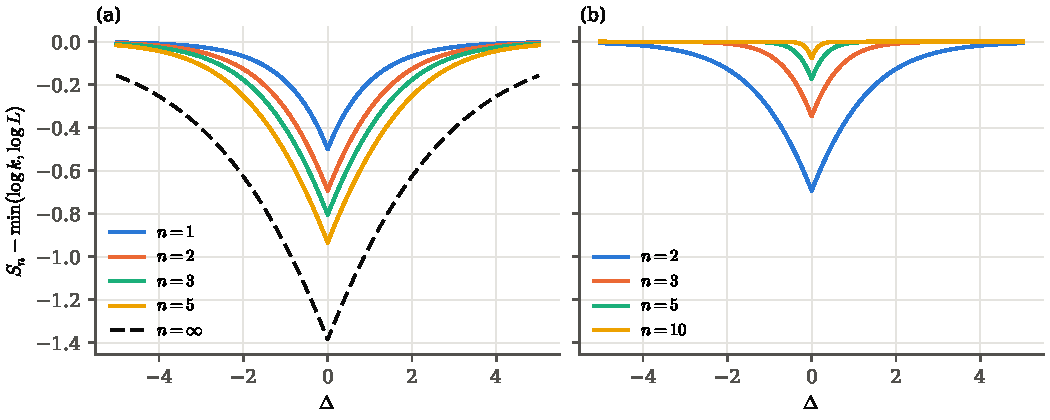
\includegraphics[width=\textwidth]{figures/output/fig05_renyi.pdf}
\caption{R\'enyi entropies through the transition at fixed area. (a) The genus-zero deficit $S_n - \log\min(k,L)$ for $n = 1, 2, 3, 5$ and the min-entropy ($n = \infty$): it deepens and broadens with $n$. (b) The two-saddle approximation for $n = 2, 3, 5, 10$: it sharpens with $n$, an artifact of the truncation.}
\label{fig05:renyi}
\end{figure}

\section{Discussion}
\label{sec06:discussion}

\subsection{What the correction means}
\label{subsec06:meaning}

The diagonal approximation rests on one physical assumption: that the radiation can tell the area sectors apart, so that their contributions to its density matrix are supported on orthogonal subspaces. \citet{marolfwangwang2020} flag this as an additional assumption, guaranteed only for sectors in which the black hole is smaller than the radiation. Theorem~\ref{thm45:limit} and its mechanism show what the assumption costs. A sector in which the black hole is smaller than the radiation occupies a subspace of the radiation of its own dimension, and different such sectors are nearly orthogonal; the radiation distinguishes them, and the entropy of mixing among them is a genuine part of its entropy. A sector in which the black hole is larger than the radiation fills the whole radiation space, as do all the others like it; the radiation cannot distinguish them, and their mixing entropy collapses into the single term $-q\log q$ for the block as a whole.

Given this distinction, the size of the correction in the broad limit does not depend on the shape of the area distribution: it is a function of one number, the canonical weight $q$ of the sectors larger than the radiation, and it is of order one in entropy units. Where the theorem applies, the correction is negligible relative to the broadening for a macroscopic black hole, with area fluctuations of order $\sqrt{S_{\mathrm{BH}}}$, so the diagonal approximation is relatively exact; it is not exact. For a Gaussian area distribution of width $\sigma = \sqrt{C_V}$ the exact planar deficit at the Page point is $-\sqrt{C_V/2\pi} + \tfrac12\log 2 + O(C_V^{-1/2})$, with the leading term the $\sqrt{C/2\pi}$ of \citet{murthysrednicki2019} and the constant missed by the diagonal approximation; for other laws the leading term is $\mathbb{E}[\min(0,\delta)]$, which is $-\sqrt{C_V/2\pi}$ only in the Gaussian case.

Whether the radiation can tell the sectors apart is a property of the model, not of the area distribution. In the west-coast model the radiation is a reference system entangled with the flavor of the end-of-the-world brane and has no energy of its own. It resolves area sectors only through the island, by reconstructing the sector of the black hole, and the island belongs to its entanglement wedge only for sectors in which the black hole is smaller than the radiation; every sector larger than the radiation fills the same space of radiation states. The situation is different when the radiation also records the sector directly. In the idealization in which the energy of each subsystem is sharp, as for an energy eigenstate of a closed system whose parts interact weakly, the energy of one subsystem fixes that of the other, the reduced density matrix of either subsystem is block diagonal in its own energy, and the sectors are orthogonal on both sides; the entropy is then the average of the fixed-energy entropies together with the full entropy of mixing, as in Eq.~(15) of \citet{murthysrednicki2019}, and no floor forms. Their result carries an uncertainty of the order of the boundary area, from the interaction between the parts, which is larger than the constant at issue here; the statement therefore concerns the idealization. \citet{marolfwangwang2020} reach the corresponding conclusion for holographic energy eigenstates, for which the off-diagonal terms vanish and the diagonal approximation should hold (their Section~6). The constant $-q\log q$ is the entropy of mixing that is lost when the radiation does not resolve the sectors larger than itself. For an evaporating black hole the energy of the Hawking radiation fluctuates by $O(\sqrt{S_{\mathrm{BH}}})$~\citep{penington2020} and, by energy conservation, is correlated with that of the black hole, so the radiation may resolve these sectors in part;
 its spectrum is then not the free compound Poisson law of Section~\ref{subsec03:canonical}, and the theorem does not apply.

\subsection{Why free probability}
\label{subsec06:why_free}

Three facts combine to make the planar replica sum a free-probability computation. The gravitational path integral is organized by topology, with genus $g$ suppressed by $e^{-2gS_0}$, so the leading order is planar. A permutation has genus zero relative to $\tau = (1\,2\,\cdots\,n)$ exactly when it is non-crossing, by the geodesic condition~\eqref{eq02:genus_zero_condition}, so the planar sum runs over $S_{\mathrm{NC}}(n) \cong \mathrm{NC}(n)$, the index set of the free moment--cumulant formula. And in the west-coast model every connection between replicas is equivalent, so a block of size $m$ carries weight $\gamma^{m-1}$: the free cumulants are $\kappa_m = \gamma^{m-1}$, and the spectrum is free Poisson. None of this involves freeness in the technical sense, which concerns several variables. Freeness enters when the black hole spectrum is itself spread out, in the canonical ensemble: the radiation spectrum is then the free multiplicative convolution of the gravitational and matter spectra~\citep{wang2023}, and the correction of Section~\ref{sec45:exact_correction} is a property of that convolution. Models with several brane types change the law $P$ of Section~\ref{subsec03:canonical} but not the planar combinatorics; bulk matter with a non-flat spectrum contributes a further free multiplicative factor~\citep{wang2023}, which lies outside the scope of Theorem~\ref{thm45:limit}.

\subsection{Implications for the Page transition}
\label{subsec06:information_paradox}

\paragraph{The transition is smooth and wide.} In the west-coast model the crossover from the Hawking saddle to the island saddle has a width of order $\sqrt{C_V}$ in entropy units. For an evaporating black hole \citet{penington2020} estimates the width from the fluctuations of order $\sqrt{S_{\mathrm{BH}}}$ in the energy of the Hawking radiation, which give a window of order $\beta\sqrt{S_{\mathrm{BH}}}$ in time; the estimate does not use the heat capacity, which for an asymptotically flat Schwarzschild black hole is negative (Section~\ref{subsec06:higher_dimensions}). For a solar-mass black hole, with $S_{\mathrm{BH}} \sim 10^{77}$, the window spans some $10^{38}$ nats, large in absolute terms and a vanishing fraction of the black hole's lifetime.

\paragraph{No sharp transition.} The saddle-point answer has a discontinuous first derivative at the Page time; the fixed-area planar answer $\log\min(k,L) - \tfrac12 e^{-|\Delta|}$ still has a cusp there; once the area fluctuates, the cusp is smoothed on the scale $\sigma$. The smoothing is a property of the exact planar answer, not only of the diagonal approximation.

\paragraph{Partially connected geometries are essential.} At fixed area the smooth crossover requires all $C_n$ non-crossing permutations, not only the identity and $\tau$. At the Page time the ratio of the full genus-zero sum to the two-saddle truncation is $C_n/2$, growing as $4^n/(2\sqrt{\pi}\,n^{3/2})$; and the R\'enyi entropies at genus zero broaden with $n$, where the truncation would make them sharpen (Section~\ref{subsec05:renyi}).

\paragraph{The entropy lies below the minimum.} Both the fixed-area deficit and the broadening of the minimum lower the entropy below $\min(S_{\mathrm{rad}}, \langle S_{\mathrm{BH}}\rangle)$. The exact correction raises it by $-q\log q \le 1/e$, while at the Page point the deficit itself is of order $\sigma$. The exact planar entropy never exceeds $\log k$: by~\eqref{eq03:canonical_entropy} the deficit is $-\int u\log u\, d\nu$, which is non-positive by Jensen's inequality because $\nu$ has mean one.

\subsection{Toward higher dimensions}
\label{subsec06:higher_dimensions}

The calculations here are in JT gravity, but several results do not depend on it. The planar combinatorics, the Marchenko--Pastur spectrum at fixed area, and the fixed-area deficit $-\tfrac12 e^{-|\Delta|}$ follow from the replica structure alone. Proposition~\ref{thm45:representation} and Theorem~\ref{thm45:limit} depend only on the law $P$ of the black hole levels relative to the radiation, given that the radiation spectrum is the free compound Poisson law of Section~\ref{subsec03:canonical}, and the theorem requires only that $P$ be broad on the scale of one nat. A model of the west-coast type built on a higher-dimensional black hole, with the radiation again a reference system entangled with brane flavors, has radiation that resolves the area only through the island, by construction; it would have a radiation spectrum of the form of Section~\ref{subsec03:canonical} if its planar replica sum has the same structure, which has not been established. For a large AdS--Schwarzschild black hole $C_V \propto S_{\mathrm{BH}}$, so $\sigma \sim \sqrt{S_{\mathrm{BH}}}$ and the hypothesis of the theorem would hold at any fixed temperature in the semiclassical limit. We therefore conjecture that the broadened Page curve of such a model carries the correction $-q\log q$ on top of the diagonal approximation. Whether the broadened Page curves of the companion paper~\citep{wuebben2026higher} carry it depends in addition on whether their radiation resolves the area directly (Section~\ref{subsec06:meaning}). For asymptotically flat Schwarzschild black holes the canonical heat capacity is negative, $C_V = -2S_{\mathrm{BH}}$ in four dimensions, and the analysis must be carried out microcanonically.

The full distribution of the area in higher dimensions is not known. In JT gravity it is set by the Schwarzian mode; in four dimensions the near-horizon fluctuations of Schwarzschild or Kerr black holes involve many more modes, and computing $P(S_{\mathrm{BH}})$ exactly remains open. The theorem needs only its breadth, the first correction~\eqref{eq45:first_order_general} needs its density near the radiation entropy, and the remaining corrections are of order $\sigma^{-2}$.

\subsection{Open questions}
\label{subsec06:open_questions}

\paragraph{The approach to the limit.} The first correction~\eqref{eq45:first_order_general} is derived formally and confirmed numerically for Gaussian laws and for the skewed JT law; a bound on the remainder would make the corrected prescription~\eqref{eq45:corrected} a controlled approximation.

\paragraph{Radiation that records the area.} The constant arises because the radiation cannot resolve the sectors larger than itself, and it is absent when the radiation resolves every sector (Section~\ref{subsec06:meaning}). How the correction interpolates between these cases, when the radiation carries part of the information about the black hole's energy, is open; the radiation spectrum is then not the free compound Poisson law used here.


\paragraph{R\'enyi entropies.} With fluctuating area, the R\'enyi moments of a mixture are dominated by a single area for $n \neq 1$~\citep{marolfwangwang2020, dongwang2020}, and \citet{peningtonrath2025} derive the corresponding diagonal approximation up to $O(\log G_N)$. Whether the R\'enyi entropies carry an analogue of the constant $-q\log q$ is not known.

\paragraph{Beyond genus zero.} The genus-$g$ contribution involves permutations with $\#(\sigma) + \#(\tau^{-1}\sigma) = n + 1 - 2g$, whose number grows rapidly with $g$; the genus expansion is presumably asymptotic. The genus-one correction is $O(e^{-2S_0})$ and does not affect the planar statements of this paper.

\paragraph{Evaporating black holes.} The model fixes the ensemble of the black hole. For an evaporating black hole $S_{\mathrm{BH}}$ changes as radiation is emitted, the width of the area distribution evolves along the trajectory, and the transition is traversed dynamically.

\paragraph{The entanglement spectrum.} At fixed area the spectrum is Marchenko--Pastur, with a gap below $a_- = (1 - \sqrt{\gamma})^2$ for $\gamma < 1$, square-root edges, and an atom at zero for $\gamma > 1$. With fluctuating area the exact planar spectrum is the free compound Poisson law of Section~\ref{subsec03:canonical}; the flat floor of Section~\ref{subsec45:mechanism} is its signature near the transition. The evolution of its edges through the transition is not worked out here.

\paragraph{Factorization and typicality.} The calculation computes the annealed entropy, $-\partial_n \langle\mathrm{Tr}(\rho^n)\rangle|_{n=1}$. The quenched entropy differs by connected contributions to the variance of $\mathrm{Tr}(\rho^n)$ across the ensemble, suppressed by $e^{-S_0}$ relative to the leading moments; bounding them uniformly near $n = 1$ would make the results statements about typical black holes rather than ensemble averages~\citep{marolfmaxfield2020, saadetal2019}.


\section{Conclusion}
\label{sec07:conclusion}

The broadened Page curve has been computed by averaging the entropy of fixed-area states over the distribution of the area, following \citet{marolfwangwang2020} and, before them, \citet{murthysrednicki2019}. That prescription is correct at the order at which it was formulated. This paper determines its error at the next order, written level by level so that it does not depend on a choice of area windows, in the model where the exact planar answer is known.

The error tends to $-q\log q$, whatever the shape of the area distribution, where $q$ is the canonical weight of the black hole levels larger than the radiation; at the Page point of a symmetric distribution it is $\tfrac12\log 2$. The constant has a simple origin. The radiation distinguishes the sectors in which the black hole is smaller than itself, which occupy nearly orthogonal subspaces of it, but not those in which the black hole is larger, which all fill the same space; the entropy of mixing among the latter collapses into a single block term. The constant is implicit in earlier work: the shifted thermal spectrum of \citet{pssyetal2022} contains the block term, the two-component mixtures of \citet{akerspenington2021} exhibit it, and \citet{marolfwangwang2020} anticipate that the sectors larger than the radiation need not be orthogonal. What is established here is the value of the constant, a proof that it is the limit of the error for every area distribution that is broad on the scale of one nat, the rate of approach, derived formally and confirmed numerically, and a representation of the exact planar entropy as a single integral that makes all of these computable. The constant requires radiation that cannot tell the larger sectors apart, as in the west-coast model; where the radiation records the area, as for energy eigenstates of a closed system, the sectors are orthogonal and the entropy of mixing is fully counted.

Three consequences follow, within the class of models to which the theorem applies. The error of the diagonal approximation is additive, so its relative size vanishes for macroscopic black holes, whose area fluctuations are of order $\sqrt{S_{\mathrm{BH}}}$; the approximation is relatively exact but not exact. The exact curve is not symmetric about the Page time, even when the area distribution is: the correction is largest, equal to $1/e$, after the Page time. And the structure of the diagonal approximation below order one, including the term $E_{\mathrm{corr}}$ produced by its fixed-area kernel, is not structure of the Page curve: the exact $1/\sigma$ term at the Page point is larger by a factor of about $2.2$. The corrected prescription~\eqref{eq45:corrected}, the diagonal approximation plus the limit and its first correction, reproduces the exact planar entropy of a Gaussian area distribution at the Page point to $0.02$ nats at $\sigma = 2.5$ and to $5\times10^{-4}$ nats at $\sigma = 6.3$.

The fixed-area ingredients are of independent use. At the Page time the two-saddle truncation of the replica sum misses the $n$th R\'enyi moment by the factor $C_n/2$, and the genus-zero R\'enyi entropies broaden with $n$ rather than sharpen. The open questions are the analogue of the constant for R\'enyi entropies with fluctuating area, a rigorous control of the first correction, the size of the correction when the radiation records the area in part, and the corresponding statement for models built on black holes in higher dimensions, where the area distribution is not known exactly.


\appendix


\section{Permutation Combinatorics}
\label{app:permutation_combinatorics}

This appendix records the combinatorics behind the genus expansion of Section~\ref{sec02:pssy_model}: the non-crossing permutations for small $n$, the identification of genus zero with the non-crossing condition, and the count of genus-one permutations.

\subsection{Non-crossing permutations for small \texorpdfstring{$n$}{n}}
\label{subsecA:enumeration}

Let $\tau = (1\,2\,\cdots\,n)$ and write $\#(\sigma)$ for the number of cycles of $\sigma \in S_n$. A permutation is non-crossing if its cycles, drawn as polygons on $n$ points placed clockwise on a circle, do not cross, and each cycle is traversed in increasing cyclic order; equivalently, no two cycles $(a_1\,\cdots)$ and $(b_1\,\cdots)$ contain elements with $a_i < b_j < a_k < b_\ell$. For $n = 3$, with products composed from left to right:

\begin{center}
\begin{tabular}{c|c|c|c|c|c}
$\sigma$ & $\#(\sigma)$ & $\tau^{-1}\sigma$ & $\#(\tau^{-1}\sigma)$ & Sum & Non-crossing \\
\hline
$\mathrm{id}$ & 3 & $(1\,3\,2)$ & 1 & 4 & yes \\
$(1\,2)$ & 2 & $(1\,3)$ & 2 & 4 & yes \\
$(2\,3)$ & 2 & $(1\,2)$ & 2 & 4 & yes \\
$(1\,3)$ & 2 & $(2\,3)$ & 2 & 4 & yes \\
$(1\,2\,3)$ & 1 & $\mathrm{id}$ & 3 & 4 & yes \\
$(1\,3\,2)$ & 1 & $(1\,2\,3)$ & 1 & 2 & no
\end{tabular}
\end{center}

Five permutations satisfy $\#(\sigma) + \#(\tau^{-1}\sigma) = 4 = n+1$, and they are the non-crossing ones: one with three cycles, three transpositions, and $\tau$ itself, matching $N(3,j) = 1, 3, 1$. The sixth, $(1\,3\,2)$, has genus one. The Narayana numbers for $n \le 5$ are in Table~\ref{tab02:narayana}.

\subsection{Genus zero is non-crossing}
\label{subsecA:genus_zero_proof}

\begin{theorem}
\label{thmA:genus_zero_nc}
For $\sigma \in S_n$ let
\begin{equation}
\label{eqA:genus_formula}
g(\sigma) = \frac{n + 1 - \#(\sigma) - \#(\tau^{-1}\sigma)}{2}.
\end{equation}
Then $g(\sigma) \ge 0$, and $g(\sigma) = 0$ if and only if $\sigma \in S_{\mathrm{NC}}(n)$.
\end{theorem}

This is the geodesic characterization of non-crossing permutations due to \citet{biane1997}; see also \citet[Lecture~23]{nicaspeicher2006}. We sketch the topological argument. Put $\omega = \sigma^{-1}\tau$, the Kreweras complement, so that $\sigma\omega = \tau$ and $\#(\omega) = \#(\tau^{-1}\sigma)$. The factorization defines a bipartite ribbon graph: a black vertex for each cycle of $\sigma$, a white vertex for each cycle of $\omega$, an edge for each $i \in \{1, \ldots, n\}$ joining the cycles that contain it, and the cyclic orders at the vertices given by the cycles. The faces correspond to the cycles of $\sigma\omega = \tau$, so there is exactly one. With $V = \#(\sigma) + \#(\omega)$, $E = n$ and $F = 1$, the Euler characteristic is
\begin{equation}
\label{eqA:euler_char}
\chi = \#(\sigma) + \#(\tau^{-1}\sigma) - n + 1 = 2 - 2g(\sigma),
\end{equation}
which is~\eqref{eqA:genus_formula} and the classical genus formula for a factorization of an $n$-cycle into two permutations~\citep{jacques1968}. The graph is planar exactly when its cycles can be drawn without crossing on the disk bounded by the single face, which is the non-crossing condition. Consequently $\#(\sigma) + \#(\tau^{-1}\sigma) \le n + 1$, with equality exactly on $S_{\mathrm{NC}}(n)$, and $0 \le g(\sigma) \le \lfloor (n-1)/2 \rfloor$.

\subsection{The genus-one count}
\label{subsecA:genus_one}

\begin{proposition}[\citealp{goupilschaeffer1998}]
\label{thmA:genus_one_count}
The number of $\sigma \in S_n$ with $g(\sigma) = 1$, that is with $\#(\sigma) + \#(\tau^{-1}\sigma) = n - 1$, is
\begin{equation}
\label{eqA:genus_one_formula}
g_1(n) = \binom{2n-2}{n-1} \frac{(n-1)(n-2)}{12}.
\end{equation}
\end{proposition}

The count is classical. A permutation $\sigma$ with $\#(\sigma) + \#(\tau^{-1}\sigma) = n + 1 - 2g$ is a factorization $\tau = \sigma\,(\sigma^{-1}\tau)$ of the long cycle of genus $g$, equivalently a rooted bicolored unicellular map with $n$ edges, and \citet{goupilschaeffer1998} enumerate these for every genus; \eqref{eqA:genus_one_formula} is their genus-one case. \citet{corihetyei2014} rederive it, refined by the number of cycles of $\sigma$, and the sequence is A002802 of the OEIS~\citep{oeisA002802}, with $g_1(n)$ its term of index $n - 3$. Equivalently, by the moment formula of \citet{hanlonstanleystembridge1992} for complex Gaussian matrices, $g_1(n)$ is the coefficient of $N^{-2}$ in the normalized $n$th moment of an $N \times N$ complex Wishart matrix. \citet{harer1986euler} give the analogous count for gluings of a $2n$-gon, which is a different family. We have checked~\eqref{eqA:genus_one_formula} against direct enumeration of all of $S_n$ for $n \le 9$. The full decomposition by genus is:

\begin{table}[ht]
\centering
\caption{Permutations of $S_n$ counted by genus relative to $\tau = (1\,2\,\cdots\,n)$, by direct enumeration. The genus-zero column is $C_n$ and the genus-one column agrees with~\eqref{eqA:genus_one_formula}.}
\label{tabA:comparison}
\begin{tabular}{c|rrrrr|r|r}
\hline
$n$ & $g = 0$ & $g = 1$ & $g = 2$ & $g = 3$ & $g = 4$ & $n!$ & $g_1(n)/C_n$ \\
\hline
3 & 5 & 1 & & & & 6 & 0.200 \\
4 & 14 & 10 & & & & 24 & 0.714 \\
5 & 42 & 70 & 8 & & & 120 & 1.667 \\
6 & 132 & 420 & 168 & & & 720 & 3.182 \\
7 & 429 & 2310 & 2121 & 180 & & 5040 & 5.385 \\
8 & 1430 & 12012 & 20790 & 6088 & & 40320 & 8.400 \\
9 & 4862 & 60060 & 174174 & 115720 & 8064 & 362880 & 12.353 \\
\hline
\end{tabular}
\end{table}

The ratio of genus one to genus zero is
\begin{equation}
\label{eqA:ratio_asymptotic}
\frac{g_1(n)}{C_n} = \frac{n(n-1)(n-2)(n+1)}{24(2n-1)} \sim \frac{n^3}{48} .
\end{equation}
For $n \ge 5$ the genus-one permutations outnumber the genus-zero ones, but each is suppressed by $L^{-2} = e^{-2S_0}$, so their total contribution, of order $n^3 L^{-2}/48$ relative to genus zero, is small whenever $L \gg n^{3/2}$. The non-crossing permutations are a vanishing fraction of $S_n$, since $C_n \sim 4^n/(\sqrt{\pi}\,n^{3/2})$ while $n! \sim \sqrt{2\pi n}\,(n/e)^n$, and they nonetheless carry the whole planar limit.



\section{Free Probability Derivations}
\label{app:free_probability}

This appendix provides detailed derivations supporting the free probability framework used in Section~\ref{sec03:free_probability}. We establish the equivalence between the Narayana moment formula arising from the gravitational path integral and the free Poisson distribution, derive the Marchenko-Pastur density from the R-transform, and verify the conditions of Carlson's theorem that guarantee uniqueness of the analytic continuation within the bounded-exponential-growth class.

\subsection{From Narayana Moments to Free Cumulants}
\label{subsecB:narayana_to_cumulants}

The genus-0 gravitational result for the radiation density matrix moments is the Narayana polynomial
\begin{equation}
\label{eqB:narayana_moments}
M_n(\gamma)=\sum_{j=1}^{n} N(n,j)\,\gamma^{\,n-j},
\end{equation}
with $M_1(\gamma)=\mathrm{Tr}(\rho)=1$ by density-matrix normalization.

\subsubsection*{Non-crossing moment--cumulant relation and identification of $\kappa_m$}

In free probability~\cite{nicaspeicher2006,voiculescu1991}, moments $\{M_n\}$ and free cumulants $\{\kappa_m\}$ are related by a sum over non-crossing partitions:
\begin{equation}
\label{eqB:moment_cumulant}
M_n \;=\; \sum_{\pi \in \mathrm{NC}(n)} \prod_{B\in\pi} \kappa_{|B|}.
\end{equation}
A convenient way to match~\eqref{eqB:narayana_moments} is to choose
\begin{equation}
\label{eqB:cumulants_gamma_power}
\kappa_m \;=\; \gamma^{m-1}\qquad (m\ge 1),
\end{equation}
so in particular $\kappa_1=\gamma^{0}=1$ agrees with $M_1=\mathrm{Tr}(\rho)=1$.

With~\eqref{eqB:cumulants_gamma_power}, each block $B$ contributes $\kappa_{|B|}=\gamma^{|B|-1}$, hence for a partition $\pi$ with $|\pi|$ blocks we get
\[
\prod_{B\in\pi}\kappa_{|B|}=\gamma^{\sum_B(|B|-1)}=\gamma^{n-|\pi|}.
\]
Grouping the non-crossing partitions by their number of blocks $|\pi|=j$ then yields
\[
M_n \;=\; \sum_{j=1}^{n} \Bigl(\#\{\pi\in\mathrm{NC}(n):|\pi|=j\}\Bigr)\,\gamma^{n-j}
\;=\;\sum_{j=1}^{n} N(n,j)\,\gamma^{n-j},
\]
which matches the gravitational Narayana formula~\eqref{eqB:narayana_moments} exactly. This is the precise sense in which the genus-0 gravitational moments define a (parameterized) free Poisson / Marchenko--Pastur law.

\subsubsection*{Equivalent standard free-Poisson parameterization}

A standard free-Poisson variable with rate $\lambda$ and jump size $a$ has free cumulants $\kappa_m=\lambda a^m$.
Matching~\eqref{eqB:cumulants_gamma_power} gives
\begin{equation}
\label{eqB:free_poisson_params}
\lambda=\frac{1}{\gamma},\qquad a=\gamma,
\end{equation}
so $\kappa_m=\lambda a^m=\gamma^{m-1}$ as required. (Equivalently, one may rescale variables to adopt the convention “all cumulants equal $\lambda$”; the present normalization is fixed by $\mathrm{Tr}(\rho)=1$ and is the one relevant for density-matrix moments.)

\subsubsection*{R-transform}

The $R$-transform generating function for free cumulants is
\begin{equation}
\label{eqB:r_transform_def}
R(z)=\sum_{m=1}^{\infty}\kappa_m z^{m-1}.
\end{equation}
Using $\kappa_m=\gamma^{m-1}$ gives
\begin{equation}
\label{eqB:r_transform_correct}
R(z)=\sum_{m=1}^{\infty}(\gamma z)^{m-1}=\frac{1}{1-\gamma z},
\end{equation}
which is equivalent to the standard free-Poisson form $R(z)=\lambda a/(1-a z)$ with~\eqref{eqB:free_poisson_params}. This $R$-transform leads (via Stieltjes inversion in the next subsection) to the Marchenko--Pastur density with support $[a_-,a_+]$ where $a_\pm=(1\pm\sqrt{\gamma})^2$ under the normalization $\mathrm{Tr}(\rho)=1$.

\subsection{From R-Transform to Marchenko-Pastur via Stieltjes Inversion}
\label{subsecB:stieltjes_inversion}
The derivation is standard~\citep{marchenkopastur1967, nicaspeicher2006}, and we record it in the normalization used here. The Cauchy transform $G(z) = \int f(x)\,dx/(z - x)$ of a law with $R$-transform $R$ satisfies
\begin{equation}
G(z) = \frac{1}{z - R(G(z))} .
\label{eqB:functional_relation}
\end{equation}
For $R(w) = 1/(1 - \gamma w)$, the free Poisson law with rate $1/\gamma$ and jump size $\gamma$, so that $\kappa_1 = 1$, this is the quadratic $\gamma z\,G^2 - (z + \gamma - 1)\,G + 1 = 0$. Its discriminant is $(z - a_+)(z - a_-)$ with
\begin{equation}
a_{\pm}=(1\pm\sqrt{\gamma})^2,
\label{eqB:endpoints}
\end{equation}
and the branch with $G(z) \sim 1/z$ at infinity is $G(z) = \big[(z + \gamma - 1) - \sqrt{(z - a_+)(z - a_-)}\big]/(2\gamma z)$. Stieltjes inversion, $f(x) = -\pi^{-1}\lim_{\varepsilon \to 0^+}\mathrm{Im}\,G(x + i\varepsilon)$, gives the Marchenko--Pastur density
\begin{equation}
f_{\mathrm{MP}}(x;\gamma)=\frac{\sqrt{(a_+-x)(x-a_-)}}{2\pi\gamma x}, \qquad x \in [a_-, a_+],
\label{eqB:mp_density_derived}
\end{equation}
together with an atom of weight $1 - 1/\gamma$ at $x = 0$ when $\gamma > 1$, which reflects the rank deficiency of $\rho_{\mathrm{rad}}$ when $k > L$.

\subsection{Carlson's Theorem: Statement and Verification}
\label{subsecB:carlson}

Carlson's theorem~\cite{carlson1914} provides a uniqueness result for analytic continuation from the positive integers within the bounded-exponential-growth class, which justifies the replica method's continuation from integer $n$ to real $n$.

\subsubsection*{Statement of Carlson's Theorem}

\begin{theorem}[Carlson, 1914]
\label{thmB:carlson}
Let $f(z)$ be a function satisfying:
\begin{enumerate}
\item[(i)] $f$ is analytic in the closed right half-plane $\{z \in \mathbb{C} : \mathrm{Re}(z) \geq 0\}$;
\item[(ii)] $f$ is of exponential type, $|f(z)| \leq A e^{\tau|z|}$ for some constants $A, \tau > 0$, and on the imaginary axis $|f(iy)| \leq A e^{c|y|}$ for some $c < \pi$;
\item[(iii)] $f(n) = 0$ for all non-negative integers $n \in \mathbb{Z}_{\geq 0}$.
\end{enumerate}
Then $f(z) \equiv 0$ for all $z$ in the right half-plane.
\end{theorem}

The condition $c < \pi$ is sharp: the function $f(z) = \sin(\pi z)$ is analytic, vanishes at all integers, and has type exactly $\pi$ along the imaginary axis. No condition is placed on the type along the real axis beyond its finiteness.

\subsubsection*{Verification for the Marchenko-Pastur Moments}

Define the moment function:
\begin{equation}
M(n) = \int_0^{\infty} x^n \, f_{\mathrm{MP}}(x; \gamma) \, dx
\label{eqB:moment_integral}
\end{equation}

We verify that this function satisfies the hypotheses of Carlson's theorem, so that it is the unique analytic continuation of the Narayana polynomial moments among continuations of exponential type that are bounded on the line $\mathrm{Re}(n) = 1$.


\paragraph{Condition (i): Analyticity.}

The integral~\eqref{eqB:moment_integral} is analytic in $n$ for $\mathrm{Re}(n) > -\tfrac12$, uniformly in $\gamma$. For $\gamma \neq 1$ the continuous part of the law is supported away from the origin, where $x^n$ is entire in $n$; for $\gamma = 1$ the density behaves as $x^{-1/2}$ at $x = 0$, so $x^n f_{\mathrm{MP}}$ is integrable exactly when $\mathrm{Re}(n) > -\tfrac12$. The atom at the origin present for $\gamma > 1$ contributes nothing for $\mathrm{Re}(n) > 0$. By dominated convergence $M(n)$ is analytic in $\mathrm{Re}(n) > -\tfrac12$. Agreement at the positive integers then suffices: $n \mapsto M(n+1) - \tilde M(n+1)$ is analytic on $\mathrm{Re}(n) \ge 0$ and vanishes at $n = 0, 1, 2, \ldots$.

\paragraph{Condition (ii): Growth Bound.}

For $\mathrm{Re}(z) \ge 0$ the shifted moment is bounded by
\begin{equation}
|M(1+z)| \leq \int_{0}^{a_+} x^{1 + \mathrm{Re}(z)} f_{\mathrm{MP}}(x) \, dx \leq a_+^{\mathrm{Re}(z)} \int_0^{a_+} x\, f_{\mathrm{MP}}(x)\, dx = a_+^{\mathrm{Re}(z)} ,
\label{eqB:moment_bound}
\end{equation}
since the law has mean one and $x \leq a_+$ on its support. Hence $M(1+z)$ has exponential type at most
\begin{equation}
\log a_+ = \log(1 + \sqrt{\gamma})^2 = 2\log(1 + \sqrt{\gamma}),
\label{eqB:exponential_type}
\end{equation}
and on the imaginary axis $|M(1+iy)| \le 1$, so its type there is zero. The hypotheses of Carlson's theorem hold for every $\gamma$.

\paragraph{Condition (iii): Agreement at Positive Integers.}

At positive integers $n = 1, 2, 3, \ldots$, the moment integral $M(n)$ computes the $n$-th moment of the Marchenko-Pastur distribution. By the free probability derivation (Section~\ref{subsecB:narayana_to_cumulants}), these moments equal the Narayana polynomial:
\begin{equation}
M(n) = \sum_{j=1}^{n} N(n, j) \, \gamma^{n-j} \quad \text{for } n \in \mathbb{Z}_{> 0}
\end{equation}

\paragraph{Uniqueness Conclusion.}

Suppose $\tilde{M}(n)$ is another analytic continuation of the Narayana moments, of exponential type in $\mathrm{Re}(n) \ge 1$ and bounded on the line $\mathrm{Re}(n) = 1$. Then $f(z) = M(1+z) - \tilde{M}(1+z)$ satisfies all conditions of Carlson's theorem, hence $f \equiv 0$, implying $\tilde{M} = M$. That is, the continuation is unique within this class, for every $\gamma$.

Therefore, the Marchenko--Pastur moment integral~\eqref{eqB:moment_integral} is the unique analytic continuation of the gravitational Narayana moments to real (and complex) R\'enyi index $n$ within that class, for every $\gamma$.

At the Page time, $\gamma = 1$, the exponential type is $\log 4$; there
 $M_n = C_n \sim 4^n/(\sqrt{\pi}\,n^{3/2})$, so $M_n/a_+^n$ decreases to zero, and $M_{100}/4^{100} = 5.58 \times 10^{-4}$.

\subsection{Proof of Proposition~\ref{prop03:exact_deficit}: the Exact Deficit}
\label{subsecB:exact_deficit}

We prove the identity~\eqref{eq03:mp_entropy_identity}. Write the Marchenko--Pastur density of mean $1$ as
\begin{equation}
\label{eqB:mp_for_proof}
\nu_\gamma(x) = \frac{\sqrt{(b-x)(x-a)}}{2\pi\gamma x}, \qquad a = (1-\sqrt{\gamma})^2, \quad b = (1+\sqrt{\gamma})^2,
\end{equation}
on $[a,b]$, supplemented for $\gamma > 1$ by an atom of mass $1 - 1/\gamma$ at the origin. The atom contributes nothing to $\int x \log x \, d\nu_\gamma$, so in both cases
\begin{equation}
\label{eqB:J_definition}
\int x \log x \, d\nu_\gamma(x) = \frac{1}{2\pi\gamma} \int_a^b \sqrt{(b-x)(x-a)} \, \log x \, dx =: \frac{I_\gamma}{2\pi\gamma}.
\end{equation}
Note that the factor of $x$ in the numerator has cancelled the $x$ in the denominator of~\eqref{eqB:mp_for_proof}; this is what makes the integral elementary.

Set $c = \tfrac{1}{2}(a+b)$ and $r = \tfrac{1}{2}(b-a)$ and substitute $x = c + r\cos\theta$, $\theta \in [0,\pi]$, so that $\sqrt{(b-x)(x-a)} = r\sin\theta$ and $dx = -r\sin\theta \, d\theta$. Then
\begin{equation}
\label{eqB:J_angular}
I_\gamma = r^2 \int_0^\pi \sin^2\theta \, \log(c + r\cos\theta) \, d\theta .
\end{equation}
Writing $c + r\cos\theta = \frac{r}{2t}\left(1 + 2t\cos\theta + t^2\right)$ with $t$ the root of $t^2 - 2(c/r)t + 1 = 0$ inside the unit disc,
\begin{equation}
\label{eqB:t_root}
t = \frac{c - \sqrt{c^2-r^2}}{r},
\end{equation}
and using the standard expansion $\log(1 - 2s\cos\theta + s^2) = -2\sum_{n\ge1} \frac{s^n}{n}\cos n\theta$ at $s = -t$,
\begin{equation}
\label{eqB:log_fourier}
\log(c + r\cos\theta) = \log\!\left(\frac{r}{2t}\right) + 2\sum_{n\ge1} \frac{(-1)^{n+1} t^n}{n} \cos n\theta .
\end{equation}
Since $\int_0^\pi \sin^2\theta \, d\theta = \pi/2$ and $\int_0^\pi \cos(n\theta)\sin^2\theta \, d\theta = -\tfrac{\pi}{4}\delta_{n,2}$, only the $n=2$ term of the sum survives, contributing $(-t^2)(-\pi/4) = \pi t^2/4$. Hence
\begin{equation}
\label{eqB:J_evaluated}
I_\gamma = r^2\left[\frac{\pi}{2}\log\!\left(\frac{r}{2t}\right) + \frac{\pi}{4}t^2\right],
\qquad
\int x \log x \, d\nu_\gamma = \frac{r^2}{2\gamma}\left[\frac{1}{2}\log\!\left(\frac{r}{2t}\right) + \frac{t^2}{4}\right].
\end{equation}

It remains to insert the Marchenko--Pastur values. From $a = (1-\sqrt\gamma)^2$ and $b = (1+\sqrt\gamma)^2$,
\begin{equation}
\label{eqB:mp_c_r}
c = 1 + \gamma, \qquad r = 2\sqrt{\gamma}, \qquad c^2 - r^2 = (1-\gamma)^2 .
\end{equation}
For $\gamma \le 1$ we have $\sqrt{c^2-r^2} = 1-\gamma$, so $t = \big[(1+\gamma)-(1-\gamma)\big]/2\sqrt{\gamma} = \sqrt{\gamma}$ and therefore
\begin{equation}
\label{eqB:collapse_small}
\frac{r}{2t} = \frac{2\sqrt{\gamma}}{2\sqrt{\gamma}} = 1 ,
\end{equation}
so the logarithm in~\eqref{eqB:J_evaluated} vanishes identically and
\begin{equation}
\label{eqB:result_small}
\int x \log x \, d\nu_\gamma = \frac{4\gamma}{2\gamma}\cdot\frac{\gamma}{4} = \frac{\gamma}{2}.
\end{equation}
For $\gamma \ge 1$ we have $\sqrt{c^2-r^2} = \gamma-1$, so $t = 1/\sqrt{\gamma}$, $r/2t = \gamma$ and $t^2 = 1/\gamma$, giving
\begin{equation}
\label{eqB:result_large}
\int x \log x \, d\nu_\gamma = \frac{4\gamma}{2\gamma}\left[\frac{1}{2}\log\gamma + \frac{1}{4\gamma}\right] = \log\gamma + \frac{1}{2\gamma}.
\end{equation}
This is~\eqref{eq03:mp_entropy_identity}. The two branches agree at $\gamma = 1$, both giving $\tfrac12$.

For the deficit, recall $S_{\mathrm{vN}} = -\int x\log x\, d\nu_\gamma + \log k$ and $\Delta = \log\gamma$. When $\gamma \le 1$, $\min(k,L) = k$ and $\mathcal{F} = -\gamma/2 = -\tfrac12 e^{\Delta}$. When $\gamma \ge 1$, $\min(k,L) = L$ and $\log k - \log L = \log\gamma$, so $\mathcal{F} = -\log\gamma - 1/(2\gamma) + \log\gamma = -1/(2\gamma) = -\tfrac12 e^{-\Delta}$. Both cases are $\mathcal{F}(\Delta) = -\tfrac12 e^{-|\Delta|}$, with no remainder. \qed

The collapse is what distinguishes the identity from the asymptotic statement: the Marchenko--Pastur law is precisely the distribution for which the Fourier parameter $t$ equals $\sqrt{\gamma}$, and for $\gamma\le1$ that is exactly the value making $r/2t = 1$. A perturbation of the spectrum away from Marchenko--Pastur reinstates the logarithm and with it a correction of order one. The canonical spectrum of Section~\ref{subsec03:canonical} is such a perturbation, which is one way to see why the broadened curve does not inherit this exactness.

\subsection{Summary: The Derivation Chain}
\label{subsecB:summary}

We have established the complete chain:

\begin{enumerate}
\item \textbf{Gravitational path integral} (the west-coast model at genus-0) produces the Narayana moment formula~\eqref{eqB:narayana_moments}.

\item \textbf{Narayana moments} are equivalent to free cumulants $\kappa_m=\gamma^{m-1}$ (with $\kappa_1=1$ from $\mathrm{Tr}(\rho)=1$), i.e.\ a (parameterized) \textbf{free Poisson / Marchenko--Pastur} law.

\item \textbf{Free Poisson R-transform} $R(z) = 1/(1-\gamma z)$ yields, via Stieltjes inversion, the \textbf{Marchenko--Pastur density}~\eqref{eqB:mp_density_derived}.

\item \textbf{Carlson's theorem} implies, for every $\gamma$, uniqueness of the analytic continuation among continuations of exponential type that are bounded on the line $\mathrm{Re}(n) = 1$; within this class, the MP moment integral gives the continuation of the gravitational R\'enyi moments to real index $n$.

\item The $n \to 1$ limit of $S_n = \log k + (1-n)^{-1} \log M_n$ yields the \textbf{von Neumann entropy} of the radiation subsystem.
\end{enumerate}

This establishes that the Page curve transition function computed from the gravitational path integral matches the entanglement entropy of a random pure state drawn from the Haar measure at genus-0, with the analytic continuation controlled (under Carlson-type hypotheses) by the Marchenko--Pastur moment representation.



\section{Gaussian Broadening Integrals}
\label{app:broadening_integrals}

This appendix derives the closed form~\eqref{eq04:E_min_alt}--\eqref{eq04:E_corr}. Let $X \sim \mathcal{N}(\mu, \sigma^2)$, with $\mu = \langle S_{\mathrm{BH}}\rangle$, and $K = S_{\mathrm{rad}}$, $\Delta = K - \mu$, $z = \Delta/\sigma$.

\subsection{The broadened minimum}
\label{subsecC:broadened_min}

Splitting at $X = K$,
\begin{equation}
\label{eqC:min_split}
\mathbb{E}[\min(X, K)] = \mathbb{E}[X;\, X < K] + K\, P(X \ge K) .
\end{equation}
The truncated mean is $\mathbb{E}[X;\, X < K] = \mu\,\Phi(z) - \sigma\,\phi(z)$, from $\int_{-\infty}^{z} (\mu + \sigma t)\phi(t)\,dt$ and $\int_{-\infty}^{z} t\,\phi(t)\,dt = -\phi(z)$, and $P(X \ge K) = \Phi(-z)$. Hence
\begin{equation}
\label{eqC:min_final}
\mathbb{E}[\min(X, K)] = \mu\,\Phi(z) + K\,\Phi(-z) - \sigma\,\phi(z) = \mu + \Delta\,\Phi(-z) - \sigma\,\phi(z),
\end{equation}
which is~\eqref{eq04:E_min_alt}.

\subsection{The fixed-area correction}
\label{subsecC:pssy_correction}

With $Y = X - \mu \sim \mathcal{N}(0, \sigma^2)$, $E_{\mathrm{corr}} = -\tfrac12\,\mathbb{E}\big[e^{-|\Delta - Y|}\big]$. Splitting at $Y = \Delta$,
\begin{equation}
\label{eqC:ecorr_split}
\mathbb{E}\big[e^{-|\Delta - Y|}\big] = e^{-\Delta}\,\mathbb{E}\big[e^{Y};\, Y < \Delta\big] + e^{\Delta}\,\mathbb{E}\big[e^{-Y};\, Y > \Delta\big].
\end{equation}
Completing the square, $e^{\pm y}\phi(y/\sigma)/\sigma = e^{\sigma^2/2}\,\phi\big((y \mp \sigma^2)/\sigma\big)/\sigma$: the weight $e^{\pm Y}$ shifts the Gaussian to mean $\pm\sigma^2$ and multiplies it by $e^{\sigma^2/2}$. Therefore
\begin{equation}
\mathbb{E}\big[e^{Y};\, Y < \Delta\big] = e^{\sigma^2/2}\,\Phi\!\left(\frac{\Delta - \sigma^2}{\sigma}\right), \qquad
\mathbb{E}\big[e^{-Y};\, Y > \Delta\big] = e^{\sigma^2/2}\,\Phi\!\left(\frac{-\Delta - \sigma^2}{\sigma}\right),
\end{equation}
and
\begin{equation}
\label{eqC:ecorr_final}
E_{\mathrm{corr}}(\Delta, \sigma) = -\frac12\, e^{\sigma^2/2}\left[e^{-\Delta}\,\Phi\!\left(\frac{\Delta - \sigma^2}{\sigma}\right) + e^{\Delta}\,\Phi\!\left(\frac{-\Delta - \sigma^2}{\sigma}\right)\right],
\end{equation}
which is~\eqref{eq04:E_corr}.

\subsection{Limits}
\label{subsecC:asymptotics}

As $\sigma \to 0$, $\mathbb{E}[\min(X,K)] \to \min(\mu, K)$, and the arguments of $\Phi$ in~\eqref{eqC:ecorr_final} tend to $\pm\infty$ according to the sign of $\Delta$, so $E_{\mathrm{corr}} \to -\tfrac12 e^{-|\Delta|}$: the fixed-area result is recovered. At the Page point, $\Delta = 0$,
\begin{equation}
\label{eqC:min_large_sigma}
\mathbb{E}[\min(X, K)] - \mu = -\frac{\sigma}{\sqrt{2\pi}}, \qquad
E_{\mathrm{corr}} = -e^{\sigma^2/2}\,\Phi(-\sigma) = -\frac{1}{\sigma\sqrt{2\pi}}\left(1 - \frac{1}{\sigma^2} + O(\sigma^{-4})\right),
\end{equation}
the last by the asymptotic expansion of $\Phi(-\sigma)$. The two terms are equal at $\sigma \approx 0.75$. For large $\sigma$ at fixed $u = \Delta/\sigma$, $E_{\mathrm{corr}} = O(1/\sigma)$ and the deficit of~\eqref{eqC:min_final} from $\min(\mu, K)$ is $\sigma\big[u\,\Phi(-u) - \phi(u) - \min(u, 0)\big] = -\sigma\big[\phi(u) - |u|\,\Phi(-|u|)\big]$, which gives~\eqref{eq04:universal}.

\section{Proofs for Section~\ref{sec45:exact_correction}}
\label{app:proofs}

Throughout, $P$ is a probability law on $(0,\infty)$ with $\mathbb{E}_P[a] < \infty$, $\delta = -\log a$, $\nu$ is the free compound Poisson law with $R(w) = \mathbb{E}_P[(1 - aw)^{-1}]$, and $h$, $s$, $v_0$, $J$ are as in Proposition~\ref{thm45:representation}. Note that $0 < h < 1$ and
\begin{equation}
\label{eqD:hprime}
h'(v) = -\,\mathbb{E}\!\left[\frac{a e^{v}}{(1 + a e^{v})^2}\right] \in \big[-\tfrac14,\, 0\big).
\end{equation}

\subsection{The representation}
\label{subsecD:representation}

\emph{Step 1: a resolvent formula.} For $u > 0$, $\log u = \int_0^\infty \big[(1+s)^{-1} - (u+s)^{-1}\big] ds$. Multiply by $u$ and integrate against $\nu$. The integrand $u(u-1)/\big((1+s)(u+s)\big)$ has a constant sign on $\{u \ge 1\}$ and on $\{u < 1\}$, so Tonelli's theorem applies to each piece, and both are finite because $\int u|\log u|\, d\nu \le e^{-1} + \int u^2 d\nu = e^{-1} + 1 + \mathbb{E}_P[a]$; the second moment of a free compound Poisson law is $\kappa_1^2 + \kappa_2$, and here $\kappa_1 = 1$, $\kappa_2 = \mathbb{E}_P[a]$. With $g(s) = \int d\nu(u)/(u+s)$ and $\int u/(u+s)\, d\nu = 1 - s\,g(s)$,
\begin{equation}
\label{eqD:resolvent_formula}
\int u \log u\, d\nu = \int_0^\infty \left[\frac{1}{1+s} - 1 + s\, g(s)\right] ds .
\end{equation}

\emph{Step 2: the fixed point on the negative axis.} The Cauchy transform $G(z) = \int d\nu(u)/(z - u)$ satisfies $G(z)\big(z - R(G(z))\big) = 1$ for $z$ in an open subset of the upper half-plane; this is the fixed-point characterization of the free compound Poisson law~\citep{nicaspeicher2006, wang2023}. $G$ is analytic on $\mathbb{C}\setminus[0,\infty)$ and takes no value in $[0,\infty)$ there: it maps the upper half-plane into the lower one, the lower into the upper, and the negative axis into the negative axis. $R$ is analytic away from the set $\{1/a : a \in \mathrm{supp}\,P\} \subset (0,\infty)$ together with its closure, which lies in $[0,\infty)$. Both sides of the identity are therefore analytic on the connected open set $\mathbb{C}\setminus[0,\infty)$, and the identity theorem extends it there. At $z = -s$, with $g(s) = -G(-s) > 0$,
\begin{equation}
\label{eqD:fixed_point}
g(s) = \frac{1}{s + h\big(\log g(s)\big)} .
\end{equation}

\emph{Step 3: inversion.} $g$ is continuous and strictly decreasing on $(0,\infty)$, with $g(s) \sim 1/s$ as $s \to \infty$ and $g(0^+) = \int d\nu/u \in (0,\infty]$. Write $\lambda = \mathbb{E}_P[1/a]$ for the total mass of the L\'evy measure; then $\nu(\{0\}) = \max(0, 1 - \lambda)$, and $g(0^+) = \infty$ exactly when $\lambda \le 1$. The map $s \mapsto v(s) = \log g(s)$ is a strictly decreasing bijection of $(0,\infty)$ onto $(-\infty, \log g(0^+))$, and by~\eqref{eqD:fixed_point} its inverse is $v \mapsto s(v) = e^{-v} - h(v)$. Hence $s > 0$ on $(-\infty, \log g(0^+))$ and $s \to 0$ at the right end, so $\log g(0^+) = v_0$, the first zero of $s$ on $[0,\infty)$; $v_0 = \infty$ exactly when $\lambda \le 1$. Directly: with $g = e^{v}$,
\begin{equation}
-s'(v) = e^{-v} + h'(v) = e^{-v}\Big(1 - g^2\, \mathbb{E}\big[a/(1 + a g)^2\big]\Big),
\end{equation}
and $g^2\mathbb{E}[a/(1+ag)^2] = g\,\mathbb{E}\big[\tfrac{ag}{1+ag}\cdot\tfrac{1}{1+ag}\big] < g\,\mathbb{E}\big[\tfrac{1}{1+ag}\big] = g\,h = 1 - s\,g \le 1$ wherever $s \ge 0$, so $s$ is strictly decreasing there.

\emph{Step 4: change of variables.} Substitute $s = s(v)$ in~\eqref{eqD:resolvent_formula}. Using $s\,g = 1 - h e^{v}$,
\begin{equation}
\frac{1}{1+s} - 1 + s\,g = \frac{1}{1+s} - h e^{v} = \frac{e^{v}(1-h)(1 - h e^{v})}{1 + (1-h)e^{v}},
\end{equation}
and multiplying by $-s'(v) = e^{-v}(1 + h' e^{v})$ gives $J(v)$. This is~\eqref{eq45:FA}.

\emph{Step 5: the subtraction.} By Tonelli,
\begin{equation}
\int_{-\infty}^0 \big(1 - h(v)\big)\, dv = \mathbb{E}\!\left[\int_{-\infty}^0 \frac{a e^{v}}{1 + a e^{v}}\, dv\right] = \mathbb{E}\big[\log(1 + a)\big] = \mathbb{E}\big[\max(0,-\delta)\big] + \mathbb{E}\big[\log(1 + e^{-|\delta|})\big].
\end{equation}
Since $S_{\mathrm{planar}} - \log k = -\int J$ by~\eqref{eq03:canonical_entropy} and~\eqref{eq45:FA}, and $S_{\mathrm{diag}} - \log k = \mathbb{E}[\min(0,\delta)] - \tfrac12\mathbb{E}[e^{-|\delta|}]$ by~\eqref{eq04:level_resolved}, subtracting gives~\eqref{eq45:gap_exact}. \qed

\emph{Bounds.} For $v < 0$, the numerator of $J/(1-h)$ minus its denominator is $e^{v}\big(h'(1 - h e^{v}) - 1\big)$, of modulus at most $\tfrac54 e^{v}$, and the denominator is at least $1$; hence
\begin{equation}
\label{eqD:bound_neg}
\big|J(v) - (1 - h(v))\big| \le \tfrac54\, e^{v} \qquad (v < 0).
\end{equation}
For $0 \le v < v_0$, $h e^{v} < 1$ because $s > 0$, and $1 + h' e^{v} = -s'(v)\, e^{v} > 0$, so $0 < J(v) \le 1$.

\subsection{The broad-distribution limit}
\label{subsecD:limit}

\emph{Proof of Theorem~\ref{thm45:limit}.} Fix $\varepsilon > 0$ and write $\pi_n(M) = P_n(|\delta| \le M)$, which tends to zero for each $M$.

\emph{The two expectations.} $\mathbb{E}_n[\log(1 + e^{-|\delta|})] \le \pi_n(M)\log 2 + \log(1 + e^{-M})$ and $\mathbb{E}_n[e^{-|\delta|}] \le \pi_n(M) + e^{-M}$; choosing $M$ large and then $n$ large makes both smaller than $\varepsilon$.

\emph{Convergence of $h_n$ and $h_n'$.} Let $|v| \le V$. On $\{\delta > M\}$, $\mathrm{logistic}(\delta - v) \ge \mathrm{logistic}(M - V)$; on $\{\delta < -M\}$, $\mathrm{logistic}(\delta - v) \le \mathrm{logistic}(V - M)$. Hence
\begin{equation}
|h_n(v) - q_n| \le \pi_n(M) + 2\,\mathrm{logistic}(V - M),
\end{equation}
so $h_n \to q$ uniformly on $[-V, V]$. In the same way $|h_n'(v)| \le \tfrac14 \pi_n(M) + e^{V - M}$, so $h_n' \to 0$ uniformly on compact sets.

\emph{The endpoint.} $s_n(v) \to e^{-v} - q$ uniformly on compact sets. The limit is positive on $[0, -\log q)$, vanishes at $-\log q$, and is negative beyond it. For $\eta > 0$ and $n$ large, $s_n > 0$ on $[0, -\log q - \eta]$ and $s_n(-\log q + \eta) < 0$, so $v_0(n) \to -\log q$; in particular $v_0(n) < \infty$.

\emph{Dominated convergence.} On $v < 0$ the integrand of~\eqref{eq45:gap_exact} converges pointwise to the first line of~\eqref{eq45:J_limit} and is dominated by $\tfrac54 e^{v}$, by~\eqref{eqD:bound_neg}. On $[0, -\log q + 1]$ write the second part as $\int J_n\, \mathbb{1}_{v < v_0(n)}$; the integrand is bounded by $1$ and converges for almost every $v$ to the second line of~\eqref{eq45:J_limit} times $\mathbb{1}_{v < -\log q}$. With $u = (1-q)e^{v}$,
\begin{equation}
\int_{-\infty}^0 \frac{-(1-q)e^{v}}{1 + (1-q)e^{v}}\, dv = -\log(2 - q), \qquad
\int_0^{-\log q}\left[\frac{1}{1 + (1-q)e^{v}} - q\right] dv = \log(2-q) + q\log q,
\end{equation}
so the integral in~\eqref{eq45:gap_exact} tends to $q\log q$ and the gap to $-q\log q$. \qed

\emph{The spreading condition is needed.} If a fixed fraction of the weight remains at $|\delta| = O(1)$, the limit changes. For example, put weight $m$ on a normal law of width $0.3$ centred at $\delta = 0$ and split the remaining weight equally between two normal modes of unit width at $\delta = \pm L$. Then $q = \tfrac12$ for every $L$, and as $L \to \infty$ the gap tends to $0.2869$ for $m = 0.2$ and to $0.1919$ for $m = 0.5$, against $\tfrac12\log 2 = 0.3466$ for $m = 0$ (Appendix~\ref{app:numerical}).

\subsection{The first-order term}
\label{subsecD:first_order}

Let $\delta$ have a density $f$ with $f(0) = O(\sigma^{-1})$ and $f' = O(\sigma^{-2})$ near $0$, and $q = P(\delta > 0)$. Since $h(v) = \mathbb{E}[\mathrm{logistic}(\delta - v)]$ and $\int(\mathrm{logistic} - \mathbb{1}_{(0,\infty)}) = 0$, for $v = O(1)$
\begin{equation}
h(v) = q - v\,f(0) + O(\sigma^{-2}), \qquad h'(v) = -f(0) + O(\sigma^{-2}),
\end{equation}
the logistic smoothing entering first at $O(\sigma^{-2})$, through $f'$. For a Gaussian law, $\delta \sim \mathcal{N}(-\Delta, \sigma^2)$ with $\Delta = \theta\sigma$, one has $f(0) = \phi(\theta)/\sigma$ and $q = \Phi(-\theta)$. The endpoint contributes nothing at first order, because $J(v_0) = 0$. With $r = 1 - q$ and $u = e^{v}$, the derivatives of the integrand at $h = q$, $h' = 0$ are
\begin{equation}
\frac{\partial J}{\partial h'} = \frac{r(1 - qu)\,u}{1 + ru}, \qquad
\frac{\partial J}{\partial h} = -\frac{1 - (2q-1)u + r^2u^2}{(1 + ru)^2}, \qquad
\frac{\partial\,(J - (1-h))}{\partial h} = \frac{u}{(1 + ru)^2},
\end{equation}
so the integral in~\eqref{eq45:gap_exact} changes at first order by $f(0)\, I_1$ with
\begin{equation}
I_1 = \int_{-\infty}^{0}\left[-\frac{v\,u}{(1+ru)^2} - \frac{r(1-qu)u}{1+ru}\right] dv
+ \int_{0}^{-\log q}\left[\frac{v\,(1 - (2q-1)u + r^2u^2)}{(1+ru)^2} - \frac{r(1-qu)u}{1+ru}\right] dv .
\end{equation}
After the substitution $v = \log u$ the integrands are rational times $\log u$, and partial fractions give $q$ for the first integral and $\tfrac12\log^2 q + \log q + 1 - q$ for the second, so $I_1 = 1 + \log q + \tfrac12\log^2 q$. The two expectations in~\eqref{eq45:gap_exact} contribute $-f(0)\,\pi^2/6$ and $+f(0)$, since $\int\log(1+e^{-|x|})\,dx = \pi^2/6$ and $\int e^{-|x|}\,dx = 2$, the terms in $f'(0)$ vanishing because both integrands are even. Collecting terms gives~\eqref{eq45:first_order_general}, and~\eqref{eq45:first_order} for Gaussian laws. The expansion is formal: the remainder is not bounded here, and the numerical confirmation is described in Section~\ref{subsec45:first_order}.

\subsection{The form with area windows}
\label{subsecD:windows}

Divide the range of $\delta$ into windows $A$ of width $w$, with probability $P_A$ and black hole eigenvalue level $x_A$, so that the window has dimension $N_A = P_A/x_A$. Its fixed-area entropy is $\log k + \min(0, d_A) - \tfrac12 e^{-|d_A|}$ with $d_A = \log N_A - \log k = \delta_A + \log P_A$. For a window smaller than the radiation, $d_A < 0$, the contribution of the window to $S_D = \sum_A P_A S(A) - \sum_A P_A \log P_A$ is $P_A(\log k + \delta_A) + O(P_A e^{-|d_A|})$: the entropy of mixing cancels $\log P_A$ and leaves the level-resolved entropy $-\log x_A$. For a window larger than the radiation the contribution is $P_A\log k - P_A\log P_A + O(P_A e^{-|d_A|})$. Writing $q'$ for the total weight of the larger windows, $-\sum_{\mathrm{large}} P_A\log P_A = -q'\log q' + q' H(P\,|\,\mathrm{large})$, and therefore
\begin{equation}
S_D - q' H(P\,|\,\mathrm{large}) = \log k + \sum_{d_A < 0} P_A\,\delta_A - q'\log q' + o(1).
\end{equation}
Suppose now that $\delta$ has a smooth density $f$ of width $\sigma$. Then $\log P_A = \log(w f(\delta_A))$ is close to a constant $-\Lambda$ over the transition region, with $\Lambda \sim \log(\sigma/w)$, so the cut $d_A < 0$ is the cut $\delta_A < \Lambda$. The weight between the two cuts is $O(\Lambda/\sigma)$ and contributes $O(\Lambda^2/\sigma)$ to the sum, so $q' \to q$ and the right-hand side tends to $\log k + \mathbb{E}[\min(0,\delta)] - q\log q$, which by Theorem~\ref{thm45:limit} is the limit of $S_{\mathrm{planar}}$. This is~\eqref{eq45:mww_form}. The argument is heuristic: the remainders $O(P_A e^{-|d_A|})$ and the variation of $\log P_A$ across the transition region are estimated, not bounded. Section~\ref{subsec45:mechanism} gives the numerical check.



\section{Numerical Methods}
\label{app:numerical}

Every number and figure in the paper is produced by the scripts that accompany its source: \texttt{exact\_correction/gap.py} implements Proposition~\ref{thm45:representation} for Gaussian and for discrete laws $P$; \texttt{exact\_correction/jt.py} builds the JT law, in the pure-JT limit or with the brane factor of~\eqref{eq03:jt_model}; \texttt{exact\_correction/paper\_numbers.py} prints every value in Sections~\ref{sec45:exact_correction} and~\ref{sec05:exact_jt}, the windowed comparison of Section~\ref{subsec04:diagonal}, and the values of Section~\ref{subsecE:convergence}; \texttt{exact\_correction/paper\_figures.py} draws the figures and computes the permutation counts of Appendix~\ref{app:permutation_combinatorics} and the fit of Section~\ref{subsecE:genus1_fit}; and \texttt{exact\_correction/validate.py} runs the checks of Section~\ref{subsecE:validation}, one of which uses an independent solver for the planar spectrum, \texttt{free\_convolution\_check.py}, in the directory above.

\subsection{The planar entropy}
\label{subsecE:overview}

The exact planar entropy is computed from~\eqref{eq45:FA} and the difference from the diagonal approximation from~\eqref{eq45:gap_exact}, by adaptive quadrature in $v$ on $[-70, 0]$ and $[0, v_0]$; the integrand of~\eqref{eq45:gap_exact} is below $10^{-30}$ at the lower limit for every law used. The endpoint $v_0$ is bracketed by stepping up from $v = 0$ until $s(v)$ changes sign, and refined by bisection; whether $v_0$ is finite is decided in advance from the total L\'evy mass $\mathbb{E}_P[1/a]$, which is available in closed form. For discrete laws $h$ and $h'$ are finite sums. For a Gaussian law of $\delta$ with mean $m$ and variance $\sigma^2$,
\begin{equation}
\label{eqE:h_gaussian}
h(v) = \Phi\!\left(\frac{m - v}{\sigma}\right) + \int \big(\mathrm{logistic}(y) - \mathbb{1}_{y > 0}\big)\, \frac{1}{\sigma}\,\phi\!\left(\frac{y + v - m}{\sigma}\right) dy,
\end{equation}
whose second term is localized within $|y| \lesssim 40$ by the decay of the logistic function and is evaluated on a fixed grid; this keeps the cost independent of $\sigma$, and the computations of Section~\ref{subsec45:first_order} run to $\sigma = 400$ in seconds.

The JT law is built on the variable $u = \sqrt{2E}$, in which the measure $\rho(E)\,y(E)\,dE = \sinh(2\pi u)\,u\,e^{-\beta u^2/2}\,du/(2\pi^2)$ is smooth, on a grid extending to $2\pi/\beta + 40/\sqrt{\beta}$. With $S_0 = 0$, which only shifts $\log k$, each grid point is a level with $\delta = \beta E + \log Z_1 - \log k$ and weight $p(E)\,dE$.

\subsection{Validation}
\label{subsecE:validation}

The representation is checked against four independent computations.
\begin{enumerate}
\item \emph{Fixed area.} For a single atom, \eqref{eq45:FA} reproduces Proposition~\ref{prop03:exact_deficit} on both branches, at $\gamma = 0.05$, $0.3$, $1$, $2$ and $7$, to $10^{-16}$.
\item \emph{The fixed point in $s$.} Solving~\eqref{eqD:fixed_point} for $g(s)$ on a logarithmic grid of $4001$ points in $s \in [10^{-10}, 10^{10}]$ and integrating~\eqref{eqD:resolvent_formula} directly agrees with~\eqref{eq45:FA} to $10^{-6}$ for discrete and Gaussian laws.
\item \emph{Finite random matrices.} For a black hole with a discretized spectrum of $21$ levels and $k = 400$ to $500$, the entropy of $\rho_{\mathrm{rad}} = C\,\mathrm{diag}(x)\,C^\dagger/\mathrm{Tr}(\cdot)$, with $C$ a complex Gaussian matrix, averaged over six samples, agrees with the planar value to $1.2\times10^{-4}$, $9.1\times10^{-4}$ and $1.0\times10^{-3}$ at widths $0.6$, $1.2$ and $1.8$, consistent with corrections of order $1/k$.
\item \emph{An independent solver.} \texttt{free\_convolution\_check.py} solves the fixed point~\eqref{eq04:selfconsistent} by iteration on the negative real axis and integrates~\eqref{eqD:resolvent_formula} on a logarithmic grid, after binning the JT and brane measure into $4000$ atoms in $\log(kx)$. At the same binning it agrees with~\eqref{eq45:FA} to $7\times10^{-6}$ on the JT measure, at $\beta = 2\pi$ with $\mu = 20$ and at $\beta = 1$ with $\mu = 200$, over $\Delta \in \{-2, 0, 2\}$; the residual is the uniform discretization error of its grid, the same $7.3\times10^{-6}$ it shows against Proposition~\ref{prop03:exact_deficit} at fixed area. Its own checks reproduce the moments $m_2 = 1 + \gamma$ and $m_3 = \gamma^2 + 3\gamma + 1$ to five decimals, and the identity $S_{\mathrm{BH}} = \langle\log\rho\rangle + H(p)$ of~\eqref{eq03:mixing_identity} to $4\times10^{-16}$.
\end{enumerate}

\subsection{Broad laws and the spreading condition}
\label{subsecE:convergence}

Theorem~\ref{thm45:limit} is checked on non-Gaussian families of growing width $W$. For $\delta$ uniform on $[-0.6W, 0.4W]$, so that $q = 0.4$ and $-q\log q = 0.3665$, the gap is $0.1394$, $0.3058$ and $0.3520$ at $W = 5$, $20$ and $80$. For a skew-normal law of shape parameter $4$ and scale $W$, with $q = 0.9221$ and $-q\log q = 0.0748$, it is $0.0268$, $0.0508$ and $0.0675$. In both the approach is at the rate $\|f\|_\infty \propto 1/W$. For two groups of levels with weights $q$ and $1-q$ at $\delta = \pm L$, the gap differs from $-q\log q$ by $-6.8\times10^{-4}$, $-8.5\times10^{-4}$ and $-5.0\times10^{-4}$ at $L = 8$ for $q = 0.2$, $0.5$, $0.8$, and by at most $5.1\times10^{-7}$ at $L = 16$. The example of Appendix~\ref{subsecD:limit} in which a fraction $m$ of the weight stays near $\delta = 0$ gives $0.3466$, $0.2869$ and $0.1919$ for $m = 0$, $0.2$ and $0.5$ at $L = 32$, independent of $L$ beyond that.

\subsection{Genus-one corrections}
\label{subsecE:genus1_fit}

At $k = L$, Page's finite-dimensional formula is $\psi(L^2 + 1) - \psi(L + 1) - (L-1)/(2L) = \log L - \tfrac12 + \tfrac{7}{12}L^{-2} + O(L^{-4})$, so its departure from the planar value $\log L - \tfrac12$ is of genus-one order. Figure~\ref{figE:genus1_fit} shows the departure for $10 \le L \le 1000$; a fit gives the exponent $-2.000$.

\begin{figure}[htbp]
\centering
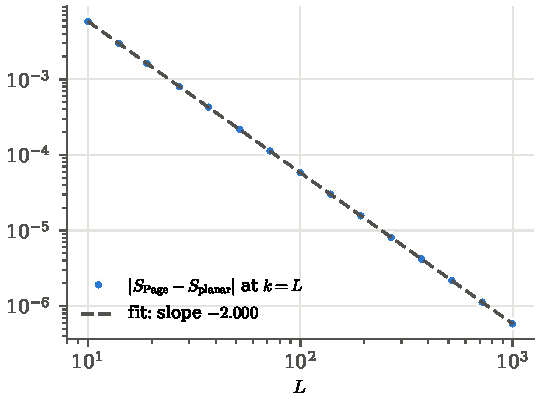
\includegraphics[width=0.5\textwidth]{figures/output/figE_genus1_fit.pdf}
\caption{The difference between Page's finite-dimensional entropy and the planar value at $k = L$, against $L$, with a power-law fit of exponent $-2.000$.}
\label{figE:genus1_fit}
\end{figure}

\subsection{Permutation counts}
\label{subsecE:permutation}

The counts of Table~\ref{tabA:comparison} are obtained by enumerating all of $S_n$ for $n \le 9$ and computing $g(\sigma)$ from~\eqref{eqA:genus_formula}; the genus-zero counts reproduce the Catalan numbers and the genus-one counts reproduce~\eqref{eqA:genus_one_formula}.


\begin{thebibliography}{99}

\bibitem[Akers et al.(2022)]{akersetal2022}
Akers, C., Faulkner, T., Lin, S., and Rath, P., 2022, The Page curve for reflected entropy, \textit{Journal of High Energy Physics} 06, 089.

\bibitem[Akers and Penington(2021)]{akerspenington2021}
Akers, C. and Penington, G., 2021, Leading order corrections to the quantum extremal surface prescription, \textit{Journal of High Energy Physics} 04, 062.


\bibitem[Almheiri et al.(2019)]{almheirietal2019}
Almheiri, A., Engelhardt, N., Marolf, D., and Maxfield, H., 2019, The entropy of bulk quantum fields and the entanglement wedge of an evaporating black hole, \textit{Journal of High Energy Physics} 12, 063.

\bibitem[Almheiri et al.(2020)]{almheirietal2020}
Almheiri, A., Hartman, T., Maldacena, J., Shaghoulian, E., and Tajdini, A., 2020, Replica wormholes and the entropy of Hawking radiation, \textit{Journal of High Energy Physics} 05, 013.

\bibitem[Bachelier(1900)]{bachelier1900}
Bachelier, L., 1900, Th\'eorie de la sp\'eculation, \textit{Annales Scientifiques de l'\'Ecole Normale Sup\'erieure} 17, 21--86.


\bibitem[Bekenstein(1973)]{bekenstein1973}
Bekenstein, J.~D., 1973, Black holes and entropy, \textit{Physical Review D} 7, 2333--2346.


\bibitem[Biane(1997)]{biane1997}
Biane, P., 1997, Some properties of crossings and partitions, \textit{Discrete Mathematics} 175, 41--53.

\bibitem[Carlson(1914)]{carlson1914}
Carlson, F., 1914, Sur une classe de s\'eries de Taylor, PhD thesis, Uppsala University.


\bibitem[Cheng et al.(2024)]{chengetal2024}
Cheng, N., C. Lancien, G. Penington, M. Walter, and F. Witteveen, 2024, Random tensor networks with non-trivial links, \textit{Annales Henri Poincar\'{e}} 25(4), 2107--2212.

\bibitem[Cori and Hetyei(2014)]{corihetyei2014}
Cori, R. and Hetyei, G., 2014, Counting genus one partitions and permutations, \textit{S\'eminaire Lotharingien de Combinatoire} 70, Article B70e, arXiv:1306.4628.

\bibitem[Dong and Wang(2020)]{dongwang2020}
Dong, X. and Wang, H., 2020, Enhanced corrections near holographic entanglement transitions: a chaotic case study, \textit{Journal of High Energy Physics} 11, 007.

\bibitem[Engelhardt and Wall(2015)]{engelhardtwall2015}
Engelhardt, N. and Wall, A.~C., 2015, Quantum extremal surfaces: holographic entanglement entropy beyond the classical regime, \textit{Journal of High Energy Physics} 01, 073.

\bibitem[Foong and Kanno(1994)]{foongkanno1994}
Foong, S.~K. and Kanno, S., 1994, Proof of Page's conjecture on the average entropy of a subsystem, \textit{Physical Review Letters} 72, 1148--1151.

\bibitem[Goupil and Schaeffer(1998)]{goupilschaeffer1998}
Goupil, A. and Schaeffer, G., 1998, Factoring $n$-cycles and counting maps of given genus, \textit{European Journal of Combinatorics} 19, 819--834.

\bibitem[Hanlon et al.(1992)]{hanlonstanleystembridge1992}
Hanlon, P.~J., Stanley, R.~P., and Stembridge, J.~R., 1992, Some combinatorial aspects of the spectra of normally distributed random matrices, \textit{Contemporary Mathematics} 138, 151--174.

\bibitem[Harer and Zagier(1986)]{harer1986euler}
Harer, J. and Zagier, D., 1986, The Euler characteristic of the moduli space of curves, \textit{Inventiones Mathematicae} 85, 457--485.


\bibitem[Hawking(1975)]{hawking1975}
Hawking, S.~W., 1975, Particle creation by black holes, \textit{Communications in Mathematical Physics} 43, 199--220.

\bibitem[Jackiw and Teitelboim(1985)]{jackiwteitelboim1985}
Jackiw, R., 1985, Lower dimensional gravity, \textit{Nuclear Physics B} 252, 343--356; Teitelboim, C., 1983, Gravitation and hamiltonian structure in two spacetime dimensions, \textit{Physics Letters B} 126, 41--45.


\bibitem[Jacques(1968)]{jacques1968}
Jacques, A., 1968, Sur le genre d'une paire de substitutions, \textit{Comptes Rendus de l'Acad\'emie des Sciences de Paris, S\'erie A} 267, 625--627.

\bibitem[Jindal and Hosur(2024)]{jindalhosur2024}
Jindal, S. and P. Hosur, 2024, Generalized free cumulants for quantum chaotic systems, \textit{Journal of High Energy Physics} 2024(9), 066.

\bibitem[Kudler-Flam and Rath(2022)]{kudlerflamrath2022}
Kudler-Flam, J. and P. Rath, 2022, Large and small corrections to the JLMS formula from replica wormholes, \textit{Journal of High Energy Physics} 2022(8), 189.

\bibitem[Lewkowycz and Maldacena(2013)]{lewkowyczmaldacena2013}
Lewkowycz, A. and Maldacena, J., 2013, Generalized gravitational entropy, \textit{Journal of High Energy Physics} 08, 090.

\bibitem[Liu and Vardhan(2021)]{liuvardhan2021}
Liu, H. and S. Vardhan, 2021, Entanglement entropies of equilibrated pure states in quantum many-body systems and gravity, \textit{PRX Quantum} 2, 010344.

\bibitem[Lloyd and Pagels(1988)]{lloydpagels1988}
Lloyd, S. and Pagels, H., 1988, Complexity as thermodynamic depth, \textit{Annals of Physics} 188, 186--213.

\bibitem[Lubkin(1978)]{lubkin1978}
Lubkin, E., 1978, Entropy of an n-system from its correlation with a k-reservoir, \textit{Journal of Mathematical Physics} 19, 1028--1031.

\bibitem[Marchenko and Pastur(1967)]{marchenkopastur1967}
Marchenko, V.~A. and Pastur, L.~A., 1967, Distribution of eigenvalues for some sets of random matrices, \textit{Mathematics of the USSR--Sbornik} 1, 457--483.

\bibitem[Marolf and Maxfield(2020)]{marolfmaxfield2020}
Marolf, D. and Maxfield, H., 2020, Transcending the ensemble: baby universes, spacetime wormholes, and the order and disorder of black hole information, \textit{Journal of High Energy Physics} 08, 044.


\bibitem[Marolf et al.(2020)]{marolfwangwang2020}
Marolf, D., S. Wang, and Z. Wang, 2020, Probing phase transitions of holographic entanglement entropy with fixed area states, \textit{Journal of High Energy Physics} 2020(12), 084.

\bibitem[M\"uck(2024)]{muck2024}
M\"uck, W., 2024, Black holes and Marchenko--Pastur distribution, \textit{Physical Review D} 109, 126001.

\bibitem[Murthy and Srednicki(2019)]{murthysrednicki2019}
Murthy, C. and M. Srednicki, 2019, Structure of chaotic eigenstates and their entanglement entropy, \textit{Physical Review E} 100, 022131.

\bibitem[Nica and Speicher(2006)]{nicaspeicher2006}
Nica, A. and Speicher, R., 2006, \textit{Lectures on the Combinatorics of Free Probability}, Cambridge University Press, Cambridge.

\bibitem[OEIS(2026)]{oeisA002802}
OEIS Foundation Inc., 2026, The On-Line Encyclopedia of Integer Sequences, sequence A002802, \url{https://oeis.org/A002802}.

\bibitem[Page(1993a)]{page1993entropy}
Page, D.~N., 1993, Average entropy of a subsystem, \textit{Physical Review Letters} 71, 1291--1294.

\bibitem[Page(1993b)]{page1993info}
Page, D.~N., 1993, Information in black hole radiation, \textit{Physical Review Letters} 71, 3743--3746.

\bibitem[Penington(2020)]{penington2020}
Penington, G., 2020, Entanglement wedge reconstruction and the information paradox, \textit{Journal of High Energy Physics} 09, 002.

\bibitem[Penington and Rath(2025)]{peningtonrath2025}
Penington, G. and Rath, P., 2025, Diagonal approximation for holographic R\'enyi entropies, \textit{Physical Review Letters} 134, 161501.

\bibitem[Penington et al.(2022)]{pssyetal2022}
Penington, G., Shenker, S.~H., Stanford, D., and Yang, Z., 2022, Replica wormholes and the black hole interior, \textit{Journal of High Energy Physics} 03, 205.

\bibitem[Ryu and Takayanagi(2006)]{ryutakayanagi2006}
Ryu, S. and Takayanagi, T., 2006, Holographic derivation of entanglement entropy from AdS/CFT, \textit{Physical Review Letters} 96, 181602.

\bibitem[Saad et al.(2019)]{saadetal2019}
Saad, P., Shenker, S.~H., and Stanford, D., 2019, JT gravity as a matrix integral, arXiv:1903.11115.

\bibitem[S\'anchez-Ruiz(1995)]{sanchezruiz1995}
S\'anchez-Ruiz, J., 1995, Simple proof of Page's conjecture on the average entropy of a subsystem, \textit{Physical Review E} 52, 5653--5655.

\bibitem[Sen(1996)]{sen1996}
Sen, S., 1996, Average entropy of a quantum subsystem, \textit{Physical Review Letters} 77, 1--3.

\bibitem[Urbach(2021)]{urbach2021}
Urbach, E.~Y., 2021, The entanglement entropy of typical pure states and replica wormholes, \textit{Journal of High Energy Physics} 2021(12), 125.

\bibitem[Vidmar and Rigol(2017)]{vidmarrigol2017}
Vidmar, L. and M. Rigol, 2017, Entanglement entropy of eigenstates of quantum chaotic Hamiltonians, \textit{Physical Review Letters} 119, 220603.

\bibitem[Voiculescu(1991)]{voiculescu1991}
Voiculescu, D., 1991, Limit laws for random matrices and free products, \textit{Inventiones Mathematicae} 104, 201--220.

\bibitem[Wang(2023)]{wang2023}
Wang, J., 2023, Beyond islands: a free probabilistic approach, \textit{Journal of High Energy Physics} 2023(10), 040.


\bibitem[Wuebben(2026)]{wuebben2026higher}
Wuebben, B.~J., 2026, The Page curve in higher dimensions: phase transitions, critical phenomena, and universal broadening, \textit{Preprint}.




\bibitem[\.{Z}yczkowski and Sommers(2001)]{zyczkowskisommers2001}
\.{Z}yczkowski, K. and H.-J. Sommers, 2001, Induced measures in the space of mixed quantum states, \textit{Journal of Physics A: Mathematical and General} 34(35), 7111--7125.

\end{thebibliography}

\end{document}
